\documentclass[
    headings=optiontotocandhead,% Erweiterung für das optionale Argument der
                                % Gliederungsbefehle aktiviert.
    twoside,
    numbers=noenddot,% Keine Punkte am Ende der Gliederungsnummern und davon
                     % abgeleiteten Nummern
    toc= %Flache TOC
    12pt, % Schriftgröße 
    titlepage, % es wird eine Titelseite verwendet 
    parskip=false, % Abstand zwischen Absätzen (ganze Zeile) 
    listof=totoc, % Verzeichnisse im Inhaltsverzeichnis aufführen 
    listof=flat, % mehr Abstand für grosse Zahlen
    numbers=noenddot, % kein Punkt am Ende bei N7ummern 
    %%enlargefirstpage,% Gibt es bei scrartcl nicht!!!!
    bibliography=totoc, % Literaturverzeichnis im Inhaltsverzeichnis aufführen 
    %index=totoc, % Index im Inhaltsverzeichnis aufführen 
    %captions=tableheading, % Beschriftung von Tabellen für Ausgabe oberhalb
                           % der Tabelle formatieren 
    %draft % Status des Dokuments (final/draft) draft hinzufügen zum anziegen 
    %%der zeilen ende
    a4paper,DIV=14,
    BCOR=15mm,
    % captions=tablesignature,
]{scrbook}

\setcounter{secnumdepth}{3}

\usepackage[T1]{fontenc}
\usepackage[utf8]{inputenc}

\usepackage[english, ngerman]{babel} % your native language must be the last one!!

\usepackage{lastpage}
\usepackage{listings}
\usepackage{blindtext}

%% Aufzählungen nicht so weit einrücken
\usepackage[inline]{enumitem}
%\setitemize{leftmargin=*} 
% Listen etwas wenige einrücken, erfordert enumitem
\setitemize{leftmargin=*}

\usepackage{lmodern}

\usepackage{xspace}

\usepackage{graphicx}

%%? \usepackage{textcomp}
\usepackage[hyphens]{url}
\usepackage{makeidx}
\makeindex
%%? \usepackage{graphicx}
\usepackage[numbers]{natbib}
\PassOptionsToPackage{normalem}{ulem}
\usepackage{ulem}

\usepackage{needspace}

\setlength\partopsep{0.5ex}%schoenere Listen
\usepackage[bottom]{footmisc}%fussnote ganz unten

\usepackage[]{microtype}
\UseMicrotypeSet[protrusion]{basicmath} % disable protrusion for tt fonts

\usepackage{multirow}   % Allows table elements to span several rows.
\usepackage{booktabs}   % Improves the typesettings of tables.
\usepackage{subcaption} % Allows the use of subfigures and enables their referencing.
\usepackage[ruled,linesnumbered,algochapter]{algorithm2e} % Enables the writing of pseudo code.
\usepackage[usenames,dvipsnames,table]{xcolor} % Allows the definition and use of colors. This package has to be included before tikz.
\usepackage{nag}       % Issues warnings when best practices in writing LaTeX documents are violated.
\usepackage{todonotes} % Provides tooltip-like todo notes.
\usepackage{float}
\usepackage{color}

%% bessere Suche im PDF
\input{glyphtounicode}
\pdfgentounicode=1
%%%%%%%%%%%%%%%%%%%%%%%%%%%%%%%%%%%%%%%%%%%%%%%%%%%%%%%%%%%%%%%%%%%%%%%%%%%%%%%%%%

%  Kopf und Fußzeilen -- links und rechts verschieden 
\newcommand{\kopfseitenummer}{{\bfseries \thepage}}
\newcommand{\kopfkapl}{{\bfseries\leftmark}}
\newcommand{\kopfkapr}{{\bfseries\rightmark}}
\newcommand{\kopfbild}{\voffset7mm
\includegraphics[width=25mm]{HTL3RLogoRGB}}
\newcommand{\kopfHTL}{Höhere Technische Bundeslehranstalt Wien 3, \\Rennweg 	Abteilung für Informationstechnologie}

\usepackage[automark,headsepline,footsepline,plainfootsepline]{scrlayer-scrpage}
%\automark[chapter]{chapter}% Eventuell wenn doppelseitig
\setkomafont{pageheadfoot}{\normalcolor\footnotesize\scshape}
\setkomafont{pagenumber}{\normalfont\normalsize}
\clearpairofpagestyles
\ihead{\headmark}
\ohead{\kopfbild}
\ifoot{\kapitelautor}
\ofoot{\pagemark}
\ModifyLayer[addvoffset=-.6ex]{scrheadings.foot.above.line}% Linie verschieben
\ModifyLayer[addvoffset=-.6ex]{plain.scrheadings.foot.above.line}% Linie verschieben
\setlength{\headheight}{32pt}

% alle Seiten mit Kopfzeile
\renewcommand{\chapterpagestyle}{scrheadings}

%% Kapitel - aufwändige Kapitelüberschriften
%Options: Sonny, Lenny, Glenn, Conny, Rejne, Bjarne, Bjornstrup
%\usepackage[Bjornstrup]{fncychap}
% Alternative: 
%\usepackage{titlesec}

% Verzeichnisse - aufwändiger
%\usepackage{tocloft}


%% Code Beispiele
%% eine Variante 
\usepackage{listings}
\renewcommand{\lstlistingname}{\inputencoding{utf8}Listing}
%% andere Variante
%\usepackage{minted}
%\setminted{
%  linenos,
%  frame=lines,
%  framesep=2mm,
%  breaklines=true
%}
% Beispiel
%\begin{listing}[H]
%\begin{minted}{bash}
%...
%\end{minted}
%\caption{Beschreibung}
%\end{listing}
%% dritte Variante 
% mit/für pandoc
% create
% pandoc -s sample.md -o sample.tex
% -> copy/paste

\usepackage{fancyvrb}
\newcommand{\VerbBar}{|}
\newcommand{\VERB}{\Verb[commandchars=\\\{\}]}
\DefineVerbatimEnvironment{Highlighting}{Verbatim}{commandchars=\\\{\}}
% Add ',fontsize=\small' for more characters per line
\newenvironment{Shaded}{}{}
\newcommand{\KeywordTok}[1]{\textcolor[rgb]{0.00,0.44,0.13}{\textbf{#1}}}
\newcommand{\DataTypeTok}[1]{\textcolor[rgb]{0.56,0.13,0.00}{#1}}
\newcommand{\DecValTok}[1]{\textcolor[rgb]{0.25,0.63,0.44}{#1}}
\newcommand{\BaseNTok}[1]{\textcolor[rgb]{0.25,0.63,0.44}{#1}}
\newcommand{\FloatTok}[1]{\textcolor[rgb]{0.25,0.63,0.44}{#1}}
\newcommand{\ConstantTok}[1]{\textcolor[rgb]{0.53,0.00,0.00}{#1}}
\newcommand{\CharTok}[1]{\textcolor[rgb]{0.25,0.44,0.63}{#1}}
\newcommand{\SpecialCharTok}[1]{\textcolor[rgb]{0.25,0.44,0.63}{#1}}
\newcommand{\StringTok}[1]{\textcolor[rgb]{0.25,0.44,0.63}{#1}}
\newcommand{\VerbatimStringTok}[1]{\textcolor[rgb]{0.25,0.44,0.63}{#1}}
\newcommand{\SpecialStringTok}[1]{\textcolor[rgb]{0.73,0.40,0.53}{#1}}
\newcommand{\ImportTok}[1]{#1}
\newcommand{\CommentTok}[1]{\textcolor[rgb]{0.38,0.63,0.69}{\textit{#1}}}
\newcommand{\DocumentationTok}[1]{\textcolor[rgb]{0.73,0.13,0.13}{\textit{#1}}}
\newcommand{\AnnotationTok}[1]{\textcolor[rgb]{0.38,0.63,0.69}{\textbf{\textit{#1}}}}
\newcommand{\CommentVarTok}[1]{\textcolor[rgb]{0.38,0.63,0.69}{\textbf{\textit{#1}}}}
\newcommand{\OtherTok}[1]{\textcolor[rgb]{0.00,0.44,0.13}{#1}}
\newcommand{\FunctionTok}[1]{\textcolor[rgb]{0.02,0.16,0.49}{#1}}
\newcommand{\VariableTok}[1]{\textcolor[rgb]{0.10,0.09,0.49}{#1}}
\newcommand{\ControlFlowTok}[1]{\textcolor[rgb]{0.00,0.44,0.13}{\textbf{#1}}}
\newcommand{\OperatorTok}[1]{\textcolor[rgb]{0.40,0.40,0.40}{#1}}
\newcommand{\BuiltInTok}[1]{#1}
\newcommand{\ExtensionTok}[1]{#1}
\newcommand{\PreprocessorTok}[1]{\textcolor[rgb]{0.74,0.48,0.00}{#1}}
\newcommand{\AttributeTok}[1]{\textcolor[rgb]{0.49,0.56,0.16}{#1}}
\newcommand{\RegionMarkerTok}[1]{#1}
\newcommand{\InformationTok}[1]{\textcolor[rgb]{0.38,0.63,0.69}{\textbf{\textit{#1}}}}
\newcommand{\WarningTok}[1]{\textcolor[rgb]{0.38,0.63,0.69}{\textbf{\textit{#1}}}}
\newcommand{\AlertTok}[1]{\textcolor[rgb]{1.00,0.00,0.00}{\textbf{#1}}}
\newcommand{\ErrorTok}[1]{\textcolor[rgb]{1.00,0.00,0.00}{\textbf{#1}}}
\newcommand{\NormalTok}[1]{#1}


%% should be last packages
\usepackage{scrhack}

\usepackage[unicode=true,
 bookmarks=true,bookmarksnumbered=false,bookmarksopen=false,
 breaklinks=true,pdfborder={0 0 0},backref=false,colorlinks=false]
 {hyperref}
\hypersetup{pdftitle={Insight},
 pdfauthor={Wer auch immer},
 pdfsubject={Diplomarbeit},
 pdfkeywords={dies, das}}
\urlstyle{same} % don't use monospace font for urls

%% for pandoc
\providecommand{\tightlist}{%
  \setlength{\itemsep}{0pt}\setlength{\parskip}{0pt}}

% Auch Fußnoten bündig ausrichten
\deffootnote[]{1em}{1em}{\textsuperscript{\thefootnotemark\ }}
%% setup
\sloppy % weniger Meldungen
\voffset7mm % etwas nach unten

%% schöner: 10000 -- gar keine, 1000 als Mittelweg
\clubpenalty = 1000 % Schusterjungen verhindern
\widowpenalty = 1000 % Hurenkinder verhindern
\displaywidowpenalty = 1000 

%%%%%%%%%%%%%%%%%%%%%%%%%%%%%%%%%%%%%%%%%%%%%%%%%%%%%%%%%%%%%%%%%%%%%%%%%%%%%%%%%%
\begin{document}
%% wir schreiben keine Umlaut mit "a "o
\shorthandoff{"}
%% mit kapitelautor kann man den Autor festlegen oder auf leer setzen - steht dann in der Fußzeile.
\newcommand{\kapitelautor}{}

%%
\newcommand{\strong}[1]{\textbf{#1}}
\newcommand{\code}[1]{\texttt{#1}}

% einfaches "siehe ..." - das Ziel muss man markieren mit \label{name} -- macht pandoc automatisch
\newcommand{\kap}[1]{Kapitel~\ref{#1}, Seite~\pageref{#1}}
\newcommand{\siehe}[1]{siehe \kap{#1}}
\newcommand{\abb}[1]{Abbildung~\ref{#1}, Seite~\pageref{#1}}

%% http://ieg.ifs.tuwien.ac.at/~aigner/download/tuwien.sty
%Div. Abkürzungen (in Anlehnung an Jochen Köpper, jkthesis):
%\RequirePackage{xspace}
\newcommand{\bzw}{bzw.\@\xspace}
\newcommand{\bzgl}{bzgl.\@\xspace}
\newcommand{\ca}{ca.\@\xspace}
\newcommand{\dah}{d.\thinspace{}h.\@\xspace}
\newcommand{\Dah}{D.\thinspace{}h.\@\xspace}
\newcommand{\ds}{d.\thinspace{}s.\@\xspace}
\newcommand{\evtl}{evtl.\@\xspace}
\newcommand{\ua}{u.\thinspace{}a.\@\xspace}
\newcommand{\Ua}{U.\thinspace{}a.\@\xspace}
\newcommand{\usw}{usw.\@\xspace}
\newcommand{\va}{v.\thinspace{}a.\@\xspace}
\newcommand{\vgl}{vgl.\@\xspace}
\newcommand{\zB}{z.\thinspace{}B.\@\xspace}
\newcommand{\ZB}{Zum Beispiel\xspace} 

%% https://github.com/Digital-Media/HagenbergThesis
\newcommand{\latex}{La\-TeX\xspace} % kein schnoerkeliges LaTeX mehr
\newcommand{\tex}{TeX\xspace}       % kein schnoerkeliges TeX mehr
\newcommand{\bs}{\textbackslash}    % Backslash character
\newcommand{\obnh}{\hskip 0pt } %optional break without hyphen: e.g. PlugIn{\obnh}Filter

\newcommand{\sa}{s.\ auch\@\xspace}
\newcommand{\so}{s.\ oben\xspace}
\newcommand{\su}{s.\ unten\@\xspace}

\newcommand{\uae}{u.\thinspace{}\"A.\@\xspace}
\newcommand{\uva}{u.\thinspace{}v.\thinspace{}a.\@\xspace}
\newcommand{\uvm}{u.\thinspace{}v.\thinspace{}m.\@\xspace}



%%%%%Anfang Titelseite
%\pagenumbering{roman}
\frontmatter % Switches to roman numbering
\title{Diplomarbeit}
\begin{titlepage}
\begin{minipage}[b]{1\columnwidth}
\parbox[b]{50mm}{
\includegraphics[width=45mm]{HTL3RLogoRGB}}
\hfill
\parbox[b]{130mm}{\footnotesize \textsc{Höhere Technische Bundeslehranstalt} Wien 3, Rennweg\\
IT \& Mechatronik\\
\\
HTL Rennweg :: Rennweg 89b\\
A-1030 Wien :: Tel +43 1 24215-10 :: Fax DW 18
}\\
\mbox{}
\end{minipage}

\vspace{1cm}


\begin{center}
\textbf{\LARGE{}Diplomarbeit}{\large{}}\\
\textbf{\large{}Insight}\\
 \vspace{15mm}
 ausgeführt an der\\
 Höheren Abteilung für Informationstechnologie/Medientechnik\\
 der Höheren Technischen Lehranstalt Wien 3 Rennweg\\
 \vspace{1cm}
 im Schuljahr 2017/2018\\
 \vspace{1cm}
 durch\\
 \vspace{0.5cm}
\textbf{\large{}Akyokus Hatice}\\
\textbf{\large{}Kienreich Niklas}\\
\textbf{\large{}Schön Kerstin}\\

\par\end{center}{\large \par}

\begin{center}
\vspace{20mm}
 \normalsize unter der Anleitung von\\
 \vspace{0.5cm}
 Mag. Roman Jerabek\\
 Mag. Andreas Fink
\par\end{center}

\begin{center}
\vspace{5mm}
Wien, \today 
\par\end{center}

\end{titlepage}%%%%%%%%%%%%%%%%%%%%% Ende Titelseite %%%%%%%%%%%%%%%%%%%%%%

\chapter*{Kurzfassung}

Was ist die Medientechnik? Was wird davon an der HTL beigebracht? \\
Mit diesen Fragen beschäftigen sich Schüler, die sich für diese Schule interessieren. Dabei haben Sie nur eine Möglichkeit sich darüber zu informieren, den Tag der offenen Tür. Am Tag der offenen Tür stehen die drei Bereiche Foto, Video und Audio im Vordergrund, wobei Webdesign, Softwareentwicklung und Webtechnik, nur kurz oder gar nicht erwähnt werden. Das große Problem hierbei ist, dass sich Interessenten an der Schule anmelden und merken, dass der Schwerpunkt bei der Programmierung liegt. Um dieses Problem zu vermeiden, entwickeln wir eine Webplattform, welche es Schülern ermöglicht sich über die Medientechnik zu informieren. Auf der Webseite befinden sich Videos sowie interaktive Elemente. Mittels Interviews werden wichtige Fragen über die Abteilung, sowie über die Schule im Allgemeinen beantwortet. Der User soll aber auch die Möglichkeit bekommen, medientechnische Elemente zu betrachten und auszuprobieren. Hierbei spielen interaktive Elemente eine große Rolle, da sie einerseits die User neugierig machen aber auch Beispiele sind, die tatsächlich beigebracht werden. Somit können sich Interessenten ein Bild von der Medientechnik machen, ohne das Missverständnisse entstehen.

\chapter*{Abstract}
\selectlanguage{english}

Thats why -- the translated text ,,Kurzfassung`` (this should be
a translation).

Im englischen Abstract sollte inhaltlich das Gleiche stehen wie in
der deutschen Kurzfassung. Versuchen Sie daher, die Kurzfassung präzise
umzusetzen, ohne aber dabei Wort für Wort zu übersetzen. Beachten
Sie bei der Übersetzung, dass gewisse Redewendungen aus dem Deutschen
im Englischen kein Pendant haben oder völlig anders formuliert werden
müssen und dass die Satzstellung im Englischen sich (bekanntlich)
vom Deutschen stark unterscheidet. Es empfiehlt sich übrigens – auch
bei höchstem Vertrauen in die persönlichen Englischkenntnisse – eine
kundige Person für das „proof reading“ zu engagieren. Die richtige
Übersetzung für „Diplomarbeit“ ist übrigens schlicht thesis, allenfalls
„diploma thesis“ oder „Master’s thesis“, auf keinen Fall aber „diploma
work“ oder gar „dissertation“\citep{hagenberg}.

Wichtig ist wegen des Abteilens ein \code{\textbackslash{}begin\{english\}}
bzw. \code{\textbackslash{}selectlanguage\{ngerman\}}.

\selectlanguage{ngerman}

\chapter*{Ehrenwörtliche Erklärung}

Ich erkläre an Eides statt, dass ich die individuelle Themenstellung
selbstständig und ohne fremde Hilfe verfasst, keine anderen als die
angegebenen Quellen und Hilfsmittel benutzt und die den benutzten
Quellen wörtlich und inhaltlich entnommenen Stellen als solche erkenntlich
gemacht habe.

\begin{flushleft}
\bigskip{}
Wien, am \today \\
\newcommand{\namesigdate}[2][8cm]{
\vspace{2cm}~\newline
\parbox{#1}{\hrule\centering #2\Large\strut}
\hfill
}
\namesigdate{Mitarbeiter Eins}
\namesigdate{Mitarbeiter Zwei} 
\namesigdate{Mitarbeiter Drei}
\par\end{flushleft}



%%%%%%%%%%%%%%%%%%%%%%%%%%%%%%%%%%%%%%%%%%%%%%%%%%%%%%%%%%%%%%%%%%%%%%%%%%%%%%%%%%%%%%%%
\cleardoublepage{}
%\setcounter{tocdepth}{2}
\tableofcontents{}
\cleardoublepage{}
\listoftables
\cleardoublepage{}
\listoffigures

%hier geht es los mit dem Text - auf einer rechten Seite
\cleardoublepage{}
%\pagenumbering{arabic}
\mainmatter







% Das komplette nächste Kapitel wird in der externen Datei diplomarbeit2.tex gespeichert. 
% Es wird an dieser Stelle im Dokument eingebaut.
% Damit ist es möglich, mehrere Personen an diverse Teile der Diplomarbeit arbeiten zu lassen.
\chapter{Das Team}
\section{Hatice Akyokus}
\section{Niklas Kienreich}
\section{Kerstin Schön}
\chapter{Das Projekt}
\renewcommand{\kapitelautor}{Autor: Hatice Akyokus}
In diesem Kapitel wird die Planung des Projektes erläutert. 

\section{Die Idee}
Am Tag der offenen Tür werden jungen Schülern gezeigt, was die Medientechnik beinhaltet. Dabei werden nur die Bereiche Video, Audio und Fotografie demonstriert. Bereiche wie Webdesign, Softwaretechnik und Webtechnologie werden gänzlich ausgelassen. Dadurch, dass die Besucher denken, dass es nur diese multimedialen Bereiche gibt, melden sie sich an und merken schnell, dass man sich erst ab der 4. Klasse auf diese Bereiche spezialisiert. Um dies zu verhindern, wurden Informationsvideos gedreht, die auf einer Webseite zur Verfügung stehen. Es wurden insgesamt fünf Videos auf die Webseite gestellt. Zwei davon sind Interviews mit dem Abteilungsvorstand der HTL Rennweg und dem Medientechniklehrer Mag. Roman Jerabek. Die übrigen Videos sorgen für den „Fun-Factor“ und sind humorvoller als die Interviews. Die Webseite beinhaltet interaktive Elemente, welche zeigen, was mit der Medientechnik gemacht werden kann. Durch diese Mittel soll gezeigt werden, was in den fünf Jahren beigebracht wird.


\section{Die Planung}

Die Projektplanung ist die wichtigste Phase eines Projektes und erfolgt nach der Definierung der Projektziele.\footnote{\label{foot:2}vgl.https://www.rechnungswesen-verstehen.de/lexikon/projektplanung.php [Zugriff: 17.03.2018]}   Weiters wird die Projektmanagementmethode und alle, für diese Methode wichtigen, Tools, welche verwendet wurden, erklärt. Im Rahmen dieser Diplomarbeit, wurde als Erstes ein Kick-Off-Meeting mit den Projektbetreuern organisiert, bei der die Durchführung besprochen wurde. Anschließend wurden, die zu erledigenden Dokumente, die Umwelt- bzw. Umfeldanalyse und die Risikoanalyse, festgelegt. Zuletzt wurde die Projektmanagementmethode festgelegt, welche für die Diplomarbeit am besten geeignet ist. Nach dem Kick-Off-Meeting wurde der Antrag, welcher die Projektziele, die Projektorganisation, die Umwelt- bzw. Umfeldanalyse, die Risikoanalyse, die Meilensteinliste, die Projektressourcen und externe Kooperationspartner enthält, geschrieben und dem Abteilungsvorstand der Informationstechnologie, Dr. Gerhard Hager, übergeben.

\section{Projektmanagement und Kommunikation}

Für diese Diplomarbeit entschied sich das Team dazu, die Projektmanagementmethode Scrum zu verwenden. Für diese Methode ist ein Tool, welches die Arbeitspakete enthält, notwendig. Hierbei verwendet das Team die Webseite taiga.io, welches mit der Webseite für Zeiterfassung, toggl.com, verwendet werden kann. Für die Dokumentenverwaltung wird Sharepoint verwendet, welche mit den HTL Rennweg Accounts verbunden sind. Dabei hat der Hauptbetreuer, sowie der Nebenbetreuer Zugriff darauf und kann alle Dokumente einsehen.

\subsection[Projektmanagementsmethode]{Projektmanagementmethode\protect\footnote{\label{foot:2}vgl.http://projektmanagement-definitionen.de/glossar/scrum/  [Zugriff: 17.03.2018]}}

Die vom Projektteam gewählte Projektmanagementmethode, ist Scrum. Scrum ist eine agile Projektmanagementmethode und wird seit den 90er Jahren in der Softwareentwicklung verwendet und findet dort seinen Ursprung. Es werden drei Rollen definiert, der Product Owner, das Entwicklungsteam und der Scrum Master. 

\subsubsection[Rollen]{Rollen\protect\footnote{\label{foot:2}vgl.https://www.scrum.de/was-macht-product-owner/ [Zugriff: 17.03.2018]} \protect\footnote{\label{foot:2}vgl.https://www.projektmagazin.de/glossarterm/entwicklungsteam-scrum [Zugriff: 17.03.2018]} \protect\footnote{\label{foot:2}vgl.http://agiles-projektmanagement.org/scrum-rollen/scrum-master/ [Zugriff: 17.03.2018]}}   
\paragraph{Product Owner}
\leavevmode \\
Der Product Owner stellt Anforderungen an das Produkt und priorisiert diese. Dabei handelt es sich immer um eine Einzelperson und keinen Ausschuss. Somit darf diese Rolle auch nicht aufgeteilt werden. Weiters, ist er für das Product Backlog zuständig und sorgt dafür, dass der Wert des Produkts maximiert wird, in dem er die Einträge maximiert und so definiert, dass das Entwicklungsteam die Einträge versteht. Er ist die einzige Person, welche Änderungen vornehmen darf und dafür rechenschaftspflichtig ist. Die Entscheidung, ob ein Sprint vorzeitig beendet werden darf, liegt ebenfalls beim Product Owner. Doch die Hauptaufgabe des Product Owners liegt darin, Rücksprache mit dem Management und Stakeholdern zu halten, um die Arbeit zu optimieren und somit eine Fortschrittskontrolle zur Erreichung des Sprintziels durchzuführen. Im Sprintreview erklärt er, welche Product-Backlog-Einträge fertig sind und welche noch zu erledigen sind. 

\paragraph{Entwicklungsteam}
\leavevmode \\
Alle Mitglieder des Entwicklungsteams sind gleichberechtigt und haben untereinander keine Hierarchie. Somit haben sie keine Weisungsbefugnisse und tragen zur Erstellung des Produktes bei. Mitglieder ohne IT-Kenntnisse werden ebenfalls als Entwickler bezeichnet. Allerdings sollte das Entwicklungsteam eine Größe zwischen drei und neun Personen betragen. Die vom Product Owner spezifizierten Einträge, werden vom Entwicklungsteam umgesetzt, wobei sie die Machbarkeit und den Aufwand der Backlog Einträge beim Sprint Planning beurteilen und über den Umfang des Backlogs entscheiden. Das Entwicklungsteam entwickelt das Produkt und ist für die Abarbeitung des Backlogs zuständig. Allerdings in einer Reihenfolge, welche vom Product Owner festgelegt wird. Am Ende eines jeden Sprints wird ein Prototyp präsentiert und über den erzielten Fortschritt berichtet. 

\paragraph{Scrum Master}
\leavevmode \\
Der Scrum Master ist kein Projektleiter, sondern dafür verantwortlich, dass die Projektmanagementmethode Srum, richtig ausgeführt wird. Falls Scrum neu eingeführt wird, ist es seine Aufgabe und Pflicht, dem restlichen Team den Ablauf zu erklären. Er trifft während des Projektablaufes keine Entscheidungen und darf nicht in Entwicklungsprozess eingreifen. Sein Aufgabenbereich liegt in der Moderation und der Vermittlung an Informationen zwischen Product Owner und dem Entwicklungsteam. Ein Scrum Master entlastet weiters das Projektteam, in dem er zentrale Aufgaben übernimmt und über die Werte und Regeln eines Projektes wacht. Weiters leitet er Meetings, in welchen er unparteiisch zu handeln hat. Somit hat ein Scrum Master Meinungsverschiedenheiten oder generelle Konflikte zu beseitigen. 

\subsubsection[Product Backlog]{Product Backlog\protect\footnote{\label{foot:2}vgl.http://scrum-fibel.de/artefakte/sprint\%20backlog.html [Zugriff: 17.03.2018}}
Der Product Backlog wird vom Product Owner angelgt, gepflegt, geordnet und priorisiert und ist eine Sammlung von Anforderungen. Das Backlog enthält „User-Stories“, welche die Bedürfnisse der Nutzer widerspiegeln. Diese enthalten grobe Anforderungen, die für das Endergebnis wichtig sind und werden beim Sprint-Planning Meeting festgelegt. Die User-Stories müssen in kleinstmögliche Aufgaben aufgegliedert werden, damit das Team diese im Sprint abarbeiten kann. Ein Sprint dauert in der Regel ein bis vier Wochen, diese wird vom Scrum Master festgelegt. Weiters spielt die Priorisierung eine wichtige Rolle, denn diese entscheidet darüber, was im nächsten Sprint abgearbeitet wird. Diese darf während dem Sprint nicht verändert werden. Allerdings werden sie in Absprache mit den Stakeholdern korrigiert und angepasst, sofern die Dringlichkeit und Notwendigkeit eine große Rolle spielen. Um einen Überblick über alle Aufgaben zu behalten, wird ein Sprint Backlog angelegt. 

\subsubsection[Sprint Backlog]{Sprint Backlog\protect\footnote{\label{foot:2}vgl.http://scrum-fibel.de/artefakte/sprint\%20backlog.html [Zugriff: 17.03.2018]}}
In einem Sprint Backlog befindet sich eine Liste von Aufgaben. Diese sind essentiell um die Anforderungen des Product Backlogs umzusetzen. Das Sprint Backlog entsteht aus der Sprint Planung, wobei der Aufwand einer Aufgabe in Stunden geschätzt wird. Die Aufgaben nimmt sich jedes Teammitglied selbst und nutzt den Sprint Backlog zur Verfolgung der Aufgaben. 

\subsubsection[Sprint Planning]{Sprint Planning\protect\footnote{\label{foot:2}vgl.http://doktor-scrum.de/sprint-planning-1/ [Zugriff: 17.03.2018]}}
Im Sprint Planning werden die Anforderungen und Arbeitspakete, die im aktuellen Sprint umgesetzt werden sollen, besprochen. Der Product-Owner organisiert alles, das Entwicklungsteam, der Scrum-Master und optional der Stakeholder, nehmen teil.  Das Sprint Planning findet zu Beginn jedes Sprints statt und dauert vier bis acht Stunden. Aus dem Product-Backlog werden eine Anzahl an höchstpriorisierten Anforderungen ausgewählt und in ein Selected-Backlog übernommen. Diese sind nur Vorschläge, denn das Entwicklerteam entscheidet letztendlich, was im Sprint realisiert werden soll. Die Sprint-Planung teilt sich in zwei Phasen auf. In der ersten Phase, werden die Anforderungen detailliert besprochen. Dabei schätzt das Entwicklungsteam den Realisationsaufwand und legt fest, was im Sprint umgesetzt wird. In der zweiten Phase bespricht das Entwicklungsteam die Realisierung und zerlegt die Anforderungen in einzelne Tasks. Bei Fragen sollte der Product Owner erreichbar sein.


\subsubsection[Daily Scrum]{Daily Scrum\protect\footnote{\label{foot:2}vgl.http://scrum-master.de/Scrum-Meetings/Daily\underline Scrum\underline Meeting [Zugriff: 17.03.2018]}}
Ein Daily Scrum-Meeting ist ein kurzes, tägliches Meeting des Teams, welches ungefähr 15 Minuten dauert. Der Scrum Master nimmt teil und greift moderierend ein, wenn nötig. Beim Daily Scrum werden Statusupdates und Geschehnisse geschildert. 

\subsubsection[Sprint Review]{Sprint Review\protect\footnote{\label{foot:2}vgl.https://www.projektmagazin.de/methoden/sprint-review [Zugriff: 18.03.2018]}}
Das Sprint Review-Meeting findet am Ende jedes Sprintes statt. Sie dient zur Einholung von Feedback von den Stakeholdern. Dabei wird das Produktinkrement vorgestellt, wobei der Stakeholder seine Meinung gibt und dadurch das Produkt im nächsten Sprint optimiert werden kann. 

\subsection{Tool für Scrum}
Taiga ist ein Open Source Tool, welches für Scrum Projekte verwendet werden kann. Durch das schlichte und moderne Design, findet man sich schnell zurecht. Man bekommt die Möglichkeit geboten entweder ein Scrum oder Kanban Template zu benutzen. In dieser Diplomarbeit wurde das Scrum Template verwendet. Taiga bietet ein Interface für das Product und Sprint Backlog und dem dazugehörigen Taskboard, welche alle Tasks grafisch darstellt und sie mit einem Status versieht, um ersichtlich zu machen, in welcher Phase sich der Task befindet. Es gibt fünf Phasen: 
\begin{itemize}
\item Neu
\item In Arbeit
\item Bereit zum Testen
\item Fertig
\item Informationen werden benötigt
\end{itemize}

Die Tasks können in die jeweilige Phase verschoben werden und sobald sie sich in der Phase „Fertig“ befinden, aktualisiert sich der Projektfortschritt. Das gibt einen genauen Überblick über den Stand des Projektes. 

\subsection{Zeiterfassung}
Für die Zeiterfassung wurde toggl.com verwendet. Durch die Eingabe des Tasks und den Klick eines Buttons, wird die Zeit aufgezeichnet und in den Reports aufgelistet. Der Projektleiter kann die erfassten Zeiten jedes Teammitgliedes sehen und auch verändern. Es gibt zwei Möglichkeiten die Zeit zu erfassen:
\begin{itemize}
\item Manual Mode
\item Timer Mode
\end{itemize}

Im Manual Mode wird die Zeit händisch eingetragen, währenddessen im Timer Mode die Zeit, ähnlich wie bei einer Stoppuhr, automatisch läuft. Das führt zu einer genaueren Zeiterfassung. 

\subsection{Kommunikationsmittel}
In der Diplomarbeit wurde teamintern WhatsApp als Kommunikationsmittel verwendet. WhatsApp ist eine Instant-Messaging-App mit der Nachrichten in Echtzeit ausgetauscht werden können. Die Projektleitung erstellte zu diesem Zwecke eine Gruppe, in welcher alle Mitglieder eingeladen wurden. In dieser Gruppe wurden wichtige Ereignisse besprochen, sowie Fragen geklärt. 
Mit den Diplomarbeitsbetreuern wurde die Kommunikation durch E-Mail bevorzugt. 

\subsection{Dokumentenverwaltung durch Sharepoint}
Für die Dokumentenverwaltung, entschied sich das Team für Microsoft Sharepoint. Dieses Tool bietet eine Verbesserung der Teamproduktivität, sowie ein bequemes Verwalten von Dokumente durch eine kurze Einarbeitungszeit und einer schnellen und leichten Erstellung einer Zusammenarbeitsumgebung. Auf Sharepoint haben das gesamte Team und die Projektbetreuer Zugriff, um hochgeladene Dateien bewerten zu können.


\chapter{Ziele}
\renewcommand{\kapitelautor}{Autor: Hatice Akyokus}
Ziel unserer Diplomarbeit ist es, Jugendlichen der Unterstufe die Medientechnik näherzubringen. Dabei greift das Team auf klassische Storytelling-Methoden zurück, welche die Spannung, und den Spaß erhöhen sollen.\\ Folgende Ziele wurden im Diplomarbeitsantrag definiert:

\section{Muss-Ziele}
\begin{enumerate}
\item RE-M 1 Webseite\\
Eine Webseite ist erstellt.\\
Auf der Webseite kann sich der Nutzer aussuchen, ob er sich nur Informationen durchlesen, oder auf eine interaktive Weise Informationen über die Schule erfahren möchte. Hierbei werden zwei Buttons angezeigt, wobei beim Klick auf einem Button ein pdf-File heruntergeladen wird, welches Informationen enthält. Die Webseite enthält interaktive Elemente, gibt dem Nutzer die Möglichkeit die Medientechnik besser kennenzulernen und ist in verschiedenen Ebenen aufgebaut.
\item RE-M 2 Videos auf der Webseite\\
Die Videos sind auf der Webseite vorhanden.
Die gedrehten Videos sind auf der Webseite ersichtlich.
\item RE-M 3 Kontaktdaten\\
Die Kontaktdaten sind auf der Webseite vorhanden.\\
Bei Fragen können sich Nutzer, per E-Mail melden. Diese wird von schulinternen Personen betreut und ist jederzeit erreichbar. Außerdem befinden sich weitere Kontaktdaten wie Adresse und Telefonnummer auf der Webseite.
\item RE-M 4 Corporate Design\\
Ein Corporate Design ist erstellt.\\
Ein Corporate Design, welche die Farben, Schriftarten und das Logo der Webseite bestimmt, wird erstellt. Diese wird als Anhaltspunkt verwendet und ist als pdf-Datei verfügbar.
\item RE-M 5 Responsive Design\\
Die Webseite ist responsive ausgeführt.\\
Die Webseite ist responsive ausgeführt und kann auf mobilen und Desktop-Geräten bedient werden. 
\item RE-M 6 Drehbuch\\
Ein Drehbuch ist für das Tag der offenen Tür und Schülervideo erstellt.\\
Ein Drehbuch wird geschrieben. Dieses beinhaltet:\\
\begin{itemize}
\item Was gefilmt wird
\item Wie es gefilmt wird
\item Gesprochener Text 
\item Gebrauchtes Equipment
\item Dresscode
\end{itemize}
\item RE-M 7 Storyboard\\
Ein Storyboard für das Animationsvideo ist erstellt.\\
Ein Storyboard für das Animationsvideo wird erstellt um die Realisierung so einfach wie möglich zu gestalten.
\item RE-M 8 Genehmigung \\
Eine Genehmigung für das Filmen ist eingeholt.\\
Eine Drehgenehmigung wird beim Direktor eingeholt. Beim Filmen in den Klassenräumen wird ebenfalls um Erlaubnis gefragt, falls Schüler auf dem Material zu sehen sein sollten.
\item RE-M 9 Fragenkatalog\\
Ein Fragenkatalog ist erstellt.\\
Ein Fragenkatalog, welches die Fragen zum Interviewen beinhaltet, wird erstellt. Dabei ist zwischen den Fragen die an einen Medientechniklehrer und denen die an den Abteilungsvorstand gestellt werden, zu unterscheiden.
\item RE-M 10 Animationsvideo \\
Ein Animationsvideo ist erstellt.\\
Das Animationsvideo ist das erste Video, welches angezeigt wird. Dieses Video thematisiert allgemeine Fakten über die Schule und die Medientechnik. Das Video soll informativ, aber auch auflockernd wirken.
\item RE-M 11 Tag der offenen Tür\\
Ein Video ist am Tag der offenen Tür gedreht.\\
Am Tag der offenen Tür werden Eltern und Kinder nach ihrem ersten Eindruck befragt und gefilmt. Dabei wird auch einen Einblick in den Tag der offenen Tür geboten. Dieses Video beinhaltet außerdem zwei Interviews. Die Szenen werden dem Drehbuch entsprechend gefilmt.
\item RE-M 12 Interview\\
Zwei Interviews sind durchgeführt.\\
Ein Medientechniklehrer und der Abteilungsvorstand der Medientechnik werden interviewt. Die Fragen werden aus dem Fragenkatalog entnommen.
\item RE-M 13 Interviewer/in\\
Zwei Interviews sind durchgeführt.\\
Ein Medientechniklehrer und der Abteilungsvorstand der Medientechnik werden interviewt. Die Fragen werden aus dem Fragenkatalog entnommen.
\item RE-M 14 Voice-Over\\
Ein Voice-Over ist vertont.\\
Das Voice-Over beinhaltet den gesprochenen Text, welcher im Drehbuch festgelegt wurde. Dieser wird ins Video in den entsprechenden Stellen eingebunden.
\item RE-M 15 Schnitt \\
Das Video ist geschnitten.\\
Das Video wird dem Drehbuch entsprechend geschnitten.
\item RE-M 16 Color-Correction\\
Color-Correction ist durchgeführt.\\
Um die Belichtung und Farbe gekonnt in Szene zu setzen, wird Color-Correction durchgeführt. Hierbei wird darauf geachtet im natürlichen Bereich zu bleiben um das Video authentisch wie möglich wirken zu lassen.
\item RE-M 17 Interview mit Schülern\\
Ein Interview mit einem ehemaligen Schüler der Schule und einem Schüler der zweiten Klasse ist durchgeführt. \\
Ein ehemaliger Schüler und ein Schüler der zweiten Klasse müssen gemeinsam Fragen beantworten und die Antwort auf eine kleine Tafel schreiben und anschließend herzeigen und die Antwort begründen.
\item RE-M 18 FAQ\\
Ein FAQ ist erstellt.\\
Auf der Webseite befinden sich FAQ’s, um häufig gestellte Fragen zu beantworten.
\item RE-M 19 Visitenkarten\\
Visitenkarten sind erstellt und ausgedruckt.\\
Es werden Visitenkarten erstellt und am Tag der offenen Türe verteilt, um Aufmerksamkeit für die Diplomarbeit zu erwecken.
\item RE-M 20 Schulleitung \\
Die Schulleitung ist in die Diplomarbeit involviert.\\
Die Kommunikation, die Planung, das rechtliche Abklären und der Einfluss in das Content-Design, erfolgt mit der Schulleitung. 
\end{enumerate}

\section{Optionale Ziele}
Dabei wurden folgende optionale Ziele festgelegt:
\begin{enumerate}
\item RE-O 1 Interaktivität erhöhen \\
Mehrere interaktive Elemente sind vorhanden.\\
Die Webseite wird ausgebaut um mehrere interaktive Elemente einzubauen. Hierbei wird dem Nutzer die Komplexität der Medientechnik gezeigt.
\item RE-O 2 Quiz\\
Ein Quiz ist erstellt.\\
Auf der ersten Ebene wird der Nutzer aufgefordert ein Quiz zu machen. In diesem Quiz kann dieser herausfinden, ob er eher für die Medientechnik oder die Netzwerktechnik geeignet ist.
\end{enumerate}
\chapter{Design}
\renewcommand{\kapitelautor}{Autor: Niklas Kienreich}

\section{Hintergedanken}
Genau, wie bei allen anderen Aspekten, dieser Diplomarbeit, war der Hintergedanke des Designs, es einladend, fröhlich und angemessen der Zielgruppe zu gestalten.

\section{Richtlinien}
\section{Corporate Design}
\subsection{Farben}
Bei den Farben wurde zum einen, ein helles Grün, zum anderen ein knalliges Orange gewählt. Als Akzentfarbe wurde ein helles Grau in das Corporate Design aufgenommen.

\subsubsection{Grün}
Wenn etwas ergrünt, ergibt sich Hoffnung auf neues Leben. Diese Farbe ist sehr naturbelassen und die Farbpsychologie lehrt, dass Grün Lebensfreude und Jugend vermittelt. Grün kann zwar auch Gift und somit eine Warnung signalisieren, durch den Kontext der Webseite ist dies aber unwahrscheinlich. \footnote{\label{foot:1} http://www.grafixerin.com/bilder/Farbpsychologie.pdf [Zugriff: 17.03.2018]}

\subsubsection{Orange}
Bei Orange handelt es sich um eine sehr auffällige Farbe. Sie ist eine warme, energiegeladene Farbe und kann aufregend, bis sogar spaßig auf einen Menschen wirken. Durch ihre Auffälligkeit kann sie aufdringlich oder extrovertiert wirken. Orange kann auch billig wirken, da der Mensch kaum etwas Hochwertiges kennt, dass diese Farbe besitzt. \footnote{\label{foot:1} http://www.grafixerin.com/bilder/Farbpsychologie.pdf [Zugriff: 17.03.2018]}

\subsubsection{Grau}
\subsection{Typografie}
\subsubsection{Parisien Night Oblique}
Diese Schrift wurde wegen ihrer dynamischen Linienführung gewählt, welche an das Logo erinnert.
\\
Verwendung findet die Schrift in den Überschriften der Website.

\subsubsection{Calibri}
Calibri ist eine serifenlose Schrift. Sie ist dadurch auf Bildschirmen mit geringerer Auflösung leicht zu lesen. Sie wirkt durch ihre abgerundeten Ecken freundlicher, als manch andere Schriftart. \footnote{\label{foot:2} https://www.typografie.info/3/Schriften/fonts.html/calibri-r61/ [Zugriff: 18.03.2018]}
\\
Calibri wird in den Texten der Website und in den Textslides der Videos verwendet.

\subsection{Adobe Illustrator}
\subsubsection{Vectorgrafiken}

\subsection{Logo}
\subsubsection{Logo-Arten}
Bei Logos unterscheidet man zwischen vier verschiedenen Arten. \footnote{\label{foot:3} http://www.webmasterpro.de/design/article/logodesign-arten-von-logos.html [Zugriff: 18.03.2018]} \footnote{\label{foot:4} http://www.sanseg.de/logodesign/zeichenmarken/ [Zugriff: 18.03.2018]}
\\
\\
Zum einen gibt es sogenannte Bildmarken. Hierbei handelt es sich um eine einfache Abbildung oder Illustration. Empfehlenswert ist solch ein Logo jedoch eher für größere Firmen und Unternehmen, da der Betrachter beim Erblicken des Logos, die Verbindung mit jenem Unternehmen herstellen können soll. Dies ist bei unbekannten Marken unwahrscheinlich und somit kontraproduktiv. Wenn ein Unternehmen auf eine Bildmarke umsteigt, gibt es oft eine Einführungsphase, in der das neue Logo anfangs mit Beschriftung gezeigt wird.
\\
\\
Eine weitere Logo-Art ist die Wortmarke. Sie zeigt einfach den Namen, des Unternehmens. Aber auch hier muss man sich Gedanken machen, wie das Logo auf den Betrachter wirkt. Neben der Farbe des Schriftzugs, sind typografische Aspekte auch wichtig. Darauf wird später in der Umsetzung des Logos genauer eingegangen.
\\
\\
Zeichenmarken sind den Wortmarken sehr ähnlich, denn sie beruhen auch auf der Typografie. Der Unterschied liegt darin, dass es sich hier nicht um Worte im Logo handelt, sondern um Abkürzungen, einzelne Buchstaben oder Zahlen.
\\
\\
Bei Wort-Bild-Marken, oder auch Kombinationen, handelt es sich, wie der Name schon verrät, um eine Kombination aus Bildmarke und entweder Wortmarke, oder Zeichenmarke. Bei dieser Art des Logos handelt es sich um die weit verbreitetste Variante. Sie ist auch am besten für kleine und mittelgroße Unternehmen geeignet.
\\
\\
Auch Keyvisuals können genutzt werden. Sie sind nicht an das Logo gebunden und können somit davon abweichen und eigene Charakteristiken veranschaulichen. Ein Keyvisual ist dann gut, wenn auf ihm der Name des Unternehmens nicht vertreten ist, der Betrachter es aber trotzdem ohne viel nachzudenken zuordnen kann.

\subsubsection{Zweck}
\subsubsection{Symbolik}
\subsubsection{Umsetzung}
\subsection{Visitenkarten}
\subsection{Designelemente}

\section{Webseite}
\subsection{Nutzen}
\subsection{Bildquellen}
\subsection{Frameworks und Libraries}
\subsubsection{Foundation}
\subsubsection{CreateJS}
\subsubsection{Timeline.js}
\subsection{Responsiveness}
\subsection{Storytelling}
\subsubsection{Story}
\subsubsection{Figur}

\subsection{Inhalt}
\subsubsection{Startseite}

\subsubsection{Interaktive Elemente}



\chapter{Video}
\renewcommand{\kapitelautor}{Autor: Kerstin Schön}
\section{Interview mit dem Abteilungsvorstand}
\subsection{Idee}
Die Intention des Interviews mit dem Abteilungsvorstand, Dr. Hager, war es, Interessenten allgemeine Informationen über die Schule näher zu bringen. Das Ziel war es, die wichtigsten Informationen kurz und prägnant rüberzubringen, sodass der Interessent die wichtigsten Informationen, ohne lang danach zu suchen, erhält.
\section{Tag der offenen Tür}
\subsection{Idee}
Das Tag der offenen Tür Video dreht sich um die Interessenten, die sich die Schule am Tag der offenen Tür angeschaut haben. Hierbei wurden Fragen, wie: "Wie ist dein erster Eindruck von der Schule?", oder "Kannst du dir vorstellen dich hier anzumelden?" gestellt. Weiters redet am Ende des Videos ein Lehrer über die Schule und erklärt den Unterschied zwischen einer HTL und einer AHS.
\section{Video mit einem Absolvent}
\subsection{Idee}
In dem Video, beziehungsweise dem Quiz, mit dem Absolventen und dem Schüler der zweiten Klasse geht es darum, dass dem Absolventen und dem Schüler Fragen gestellt werden, wobei sie 45 Sekunden Zeit haben diese zu beantworten. Derjenige, der die Frage falsch beantwortet, muss ein Jelly-Bean essen, wobei man nicht weiß, ob es ein gutes oder ein schlechtes ist. Die Intention dieses Videos ist es zu zeigen, dass die Medientechnik ein enorm großer Bereich ist, bei dem man nicht alles erlernen kann. So spezialisiert sich jeder Schüler meist auf ein Gebiet, das er dann auch dementsprechend gut kann. Was jedoch zu beachten ist, ist, dass die Schüler dennoch die Grundlagen der anderen Medientechnik Themen lernen und auch können.
\section{Technik}
\subsection{Auflösung}
Bei der Auflösung wird heutzutage unter SD, HD (2k), Digital Cinema (2k) und UHD (4k/8k) unterschieden. SD bedeutet Standard Definition und dominierte früher das Fernsehen. Heutzutage ist der Standard nicht mehr Standard Definiton, sondern High Definition. Obwohl bei Smartphones, TV-Geräten und Kameras schon Full-HD, also 1920 x 1080 px, der Vorreiter ist, wird zumindest im deutschen Fernsehen noch im normalen HD Format, also 1280 x 720 px, ausgestrahlt.\footnote{\label{}vgl. Jörg Jovy, 2017, S. 109f.}\newline
Bei den Videoaufnahmen wurde immer im Full-HD Format aufgenommen, also mit 1920 x 1080 px, da heutzutage die meisten Videos, von den Jugendlichen, am Smartphone angesehen werden.
\subsection{Aspect-Ratio - Seitenverhältnis}
Früher, als SD das Standard Fernsehformat war, war das Seitenverhältnis eines Fernsehbildes 4:3. Jedoch wurde später aus 4:3, 16:9, was auch heute im HD Format noch beibehalten wurde. Das SD Format verwendet rechteckige Pixel, was die Folge hat, dass ein SD Bild immer die gleiche Anzahl von Pixeln hat, nämlich 720 x 576. "Nur werden einmal rechteckige Pixel mit einem Seitenverhältnis von 1,46:1 (= 16:9) und einmal von 1,09:1 (= 4:3) verwendet." (Jörg Jovy, 2017, S.108)\newline 
Man nennt dies auch anamorph. "Anamorph bedeutet, dass die Pixel des Films nicht quadratisch sind, sondern rechteckig." (Jörg Jovy, 2017, S.572)\newline
Da Computer und HD-Bilder nur quadratische Pixel anzeigen, aber ein SD Fernsehformat rechteckige, muss man bei der Auswahl des Formats berücksichtigen, wo man das Video oder den Film schlussendlich abspielen möchte.\footnote{\label{}vgl. Jörg Jovy, 2017, S. 108, S. 572}
\subsection{Bildrate}
Seit 1967 wird im deutschen Fernsehen mit dem sogenannten PAL Format (=Phase Alternative Line) gesendet. Im PAL Format werden 25 Bilder pro Sekunde oder 50 Halbbilder pro Sekunde gesendet. Jedoch herrscht in den USA nicht das PAL Format, sondern das sogenannte NTSC Format (=National Television Systems Committee), welches 30 Vollbilder pro Sekunde oder 60 Halbbilder pro Sekunde sendet. Diese unterschiedlichen Bildraten sind der Tatsache geschuldet, da in Europa eine Wechselspannungsfrequenz von 50Hz herrscht, und in den USA eine von 60Hz.\footnote{\label{}vgl. https://gwegner.de/know-how/verwirrung-um-die-frameraten-24-fps-25-fps-30-fps-pal-ntsc-wann-nimmt-man-was/ [Zugriff: 17.03.2018]}\newline
Bei Videoaufnahmen wurde mit 25fps (= frames per second), also mit 25 Vollbildern in der Sekunde, aufgenommen.
\subsection{Farbraum}
Rot, Grün und Blau sind die drei Grundfarben des RGB Farbraums. Aus den drei Grundfarben bilden sich alle anderen Farben, die im RGB Farbraum möglich sind, was man RGB-Farbmischung nennt.\begin{quote}"Bei einer 8-Bit-Codierung pro Farbe stehen 256 verschiedene Farbwerte zur Verfügung. Aus der Mischung ergeben sich theoretisch 16,78 Mio. verschiedene Farbwerte (= 256 x 256 x 256)." (Jörg Jovy, 2017, S. 113)\end{quote} Schwarz enthält keine Farbinformation von den drei Grundfarben, wohingegen Weiß die Mischung aller drei Grundfarben ist. Der Farbraum des HD Standards ist RGB oder auch genannt als sRGB. Bei der Kamera kann zwischen sRGB und Adobe RGB umgestellt werden. Meist wird der Adobe RGB Farbraum, da er einen größeren Farbraum bietet. Wie man anhand der Abbildung \ref{fig:abb16} sehen kann, hat der Adobe RGB Farbraum mehr Grüntöne als der sRGB Farbraum.\footnote{\label{}vgl. Jörg Jovy, 2017, S. 112f.}
\begin{figure}[H]
\centering
	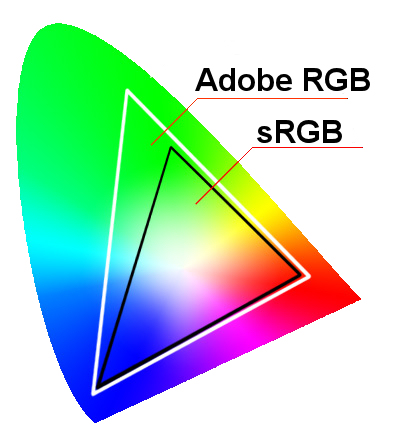
\includegraphics[width=0.3\textwidth]{abb16} 
	\caption{sRBG und Abobe RGB Farbraum}\label{fig:abb16}
\end{figure}
\subsection{Farbabtastung}
Bei der Farbabtastung handelt es sich um eine Komprimierung von  der Übertragung der Signale. Da ein unkomprimiertes Signal eine zu große Bandbreite in Anspruch nehmen würde, muss das Signal komprimiert werden. Dafür wird die Farbabtastung in Betracht gezogen. Da das menschliche Auge die Helligkeitskontraste besser auflöst als die Farbkontraste, wird bei der Farbabtastung die Helligkeit, oder Luminanz, mit der vollen Datenbreite zur Verfügung gestellt. Die Farbinformation wird, bei der Farbabtastung, jedoch reduziert. Daraus ergibt sich dann ein voll aufgelöstes Signal mit der Farbabtastung von 4:4:4. Ein bereits komprimiertes Signal hat eine Farbunterabtastung von 4:2:2, 4:2:0 oder von 4:1:1.\footnote{\label{}vgl. Jörg Jovy, 2017, S. 114.}
\paragraph{4:2:2}
\leavevmode \\
Bei der Farbunterabtastung von 4:2:2 wird bei jedem Pixel der Helligkeitswert abgetastet, wobei der Farbwert nur bei jedem zweiten Pixel abgetastet wird.\footnote{\label{}vgl. https://www.itwissen.info/Farb-Subsampling-color-subsampling.html [Zugriff: 18.03.2018]}
\paragraph{4:2:0}
\leavevmode \\
\begin{quote}"Beim Subsampling von 4:2:0, erfolgt die Abtastung der Chrominanzsignale für jeweils vier quadratisch angeordnete nebeneinander liegende Pixel. Wie bei den anderen Subsampling-Verfahren auch, wird das Luminanzsignal bei jedem Pixel abgetastet." (https://www.itwissen.info/Farb-Subsampling-color-subsampling.html [Zugriff: 18.03.2018])\end{quote}
\paragraph{4:1:1}
\leavevmode \\
Bei der Farbunterabtastung von 4:1:1 werden die Chrominanzsignale bei jeder vierter Abtastung des Helligkeitssignal abgetastet.\footnote{\label{}vgl. https://www.itwissen.info/Farb-Subsampling-color-subsampling.html [Zugriff: 18.03.2018]}
\begin{figure}[H]
	\centering	
	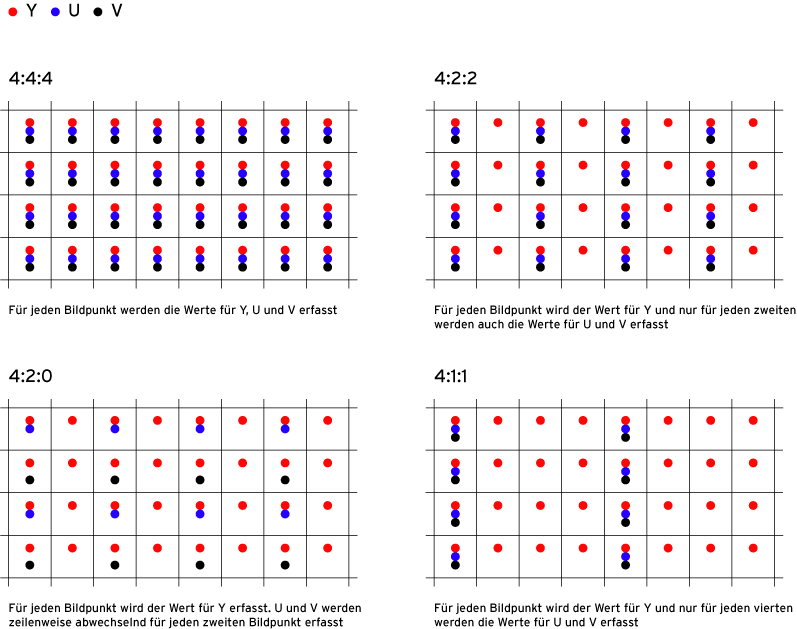
\includegraphics[width=0.8\textwidth]{abb15} 
	\caption{Farbabtastung}
\end{figure}
\subsection{Weißabgleich}
Bevor man ein Bild schießt, oder ein Video dreht, führt man zuerst einen Weißabgleich durch. Dabei wird zwischen manuellen und automatischen Weißabgleich unterschieden. Der Weißabgleich misst die derzeitige Farbtemperatur des Lichts. Die Farbtemperatur wird in Kelvin angegeben. Eine Kerze hat eine sehr rötliche und warme Farbstimmung mit einer Farbtemperatur von 1.500 Kelvin, wohingegen das Tageslicht neutral wirkt und eine Farbtemperatur von 5.000 bis 6.000 besitzt. Um den Weißabgleich manuell abzustimmen, wird ein weißes Blatt Papier vor die Kamera gehalten, und der Weißabgleich kann somit eingestellt werden. Das weiße Blatt Papier ist jedoch nur ein Hilfsmittel. Optimal wäre, eine professionelle Graukarte zu verwenden. Das Problem mit dem Papier ist, dass es optische Aufheller, die den Blauanteil erhöhen, besitzt. Das heißt, da die Kamera den zu hohen Blauanteil korrigiert, wird das Bild schlussendlich leicht gelbstichig.\footnote{\label{}vgl. Jörg Jovy, 2017, S. 201ff.}

\section{Kameramodelle}
\subsection{DSLR Kamera - Aufbau}
DSLR bedeutet Digital Single Lens Reflex und sind Spiegelreflexkameras mit digitalem Aufnahmesensor. Beispiele für eine Spiegelreflexkamera sind die Canon EOS 60D oder die Canon EOS 70D. In der folgenden Abbildung wird der Aufbau einer DSLR Kamera erklärt.\newline 
Wie man in der Abbildung \ref{fig:abb13} sehen kann, geht das Licht zuerst durch die Linse des Objektivs (1). Anschließend trifft das Licht auf den Schwingspiegel (2), welcher das Licht auf die Mattscheibe (5) reflektiert. Daraufhin verkleinert es die Sammellinse (6) auf die Größe des Suchers. Da das Bild noch spiegelverkehrt ist, spiegelt es das Pentaprisma (7) und kann so im Sucher (8) dann angezeigt werden. Als nächstes wird der Auslöser getätigt. Durch das Klicken auf den Auslöser wird der Spiegel nach oben geklappt und der Weg zum Schlitzverschluss (3) wird freigegeben. Anschließend öffnet sich dieser Verschluss und das Licht fallt auf den Sensor (4). Zum Schluss wird das Bild abgespeichert.\citep{aufbau}
\begin{figure}[H]
	\centering
	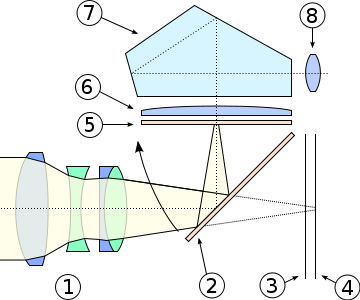
\includegraphics[width=0.6\textwidth]{abb13} 
	\caption[Aufbau einer DSLR Kamera]{Aufbau einer DSLR Kamera\footnotemark}\label{fig:abb13}
\end{figure}
\footnotetext{Quelle: http://referate.mezdata.de/sj2009/dslr\_sinan-saglam/ausarbeitung/seite2.htm}
\subsection{Sensoren}
Heutzutage gibt es zwei Vorreiter im Bereich der Sensoren. Nämlich einerseits den CMOS-Sensor und andererseits den CCD Sensor. Welcher Sensor nun auch wirklich besser ist, und in welcher Kamera welcher Sensor eingebaut werden soll, ist jedoch noch umstritten.\citep{sensor}
\paragraph{CMOS-Chips}
\leavevmode \\
Die CMOS Sensoren haben den großen Nachteil, dass das Bild bei schnellen Bewegungen, etwa wie beim Filmen von fahrenden Autos, verzerrt dargestellt wird. Dies wird auch Rolling-Shutter-Effekt genannt. Bei dem Rolling-Shutter-Effekt schauen die vertikalen Linien so aus, als würden sie umfallen, was das Bild unbrauchbar machen kann.\citep{sensor}
\paragraph{CCD-Chips}
\leavevmode \\
Die CCD Sensoren haben zwar nicht das Problem mit dem Rolling-Shutter-Effekt, jedoch sind diese Sensoren lichtempfindlicher. Das bedeutet, dass wenn das Licht direkt ins Objektiv scheint, tritt der Blooming-Effekt auf. Beim Blooming-Effekt wird das Bild von einem breiten weißen Streifen geteilt. Scheint Kunstlicht in das Objektiv, entstehen wandernde violette Streifen.\citep{ccd}
\subsection{Canon EOS 60D}
Die Canon EOS 60D DSLR (Digital Single Lens Reflex) Kamera bietet einen 18 Megapixel APS-C CMOS Sensor mit einer Größe von 22,3 mm x 14,9 mm. Die Spiegelreflexkamera nimmt mit Full HD (1920 x 1080) auf, wobei standardgemäß mit 25 Bildern pro Sekunde aufgenommen wird. Die Auflösung wird meistens mit 1080p gekennzeichnet, wobei das p für progressive steht, also für die Vollbilder.\citep{canon60}\citep{canon60Zwei}
\subsection{Canon EOS 70D}
Die Canon EOS 70D bietet einen minimal größeren Sensor im Gegensatz zu der Canon EOS 60D. Die Größe des Sensors der Canon EOS 70D beträgt 22,5 mm x 15,0 mm. Die Sensorgröße einer Kamera ist entscheidend, da folgendes gilt: "Je kleiner der Sensor, desto geringer sind die Möglichkeiten, mit einer definierten Schärfentiefe zu arbeiten." (Jörg Jovy, 2017, S. 136)\newline
Die Canon EOS 70D nimmt ebenfalls mit Full HD auf, wobei zu beachten ist, dass sie zusätzlich die Möglichkeit bietet, mit Intra-Frame oder Inter-Frame aufzunehmen.\citep{canon70} Bei Intra- oder Inter-Frames wird jedes Einzelbild komprimiert, das heißt, es kann auf jedes einzelne Bild zugegriffen werden\citep{intra}, was sich in der Post Production positiv widerspiegelt, da man keine Gruppen aus Bildern bearbeiten muss, sondern im Notfall jedes einzelne Bild bearbeiten kann. Weiters spielt bei der Wahl der richtigen Kamera, der Cropfaktor eine wichtige Rolle. "Je kleiner ein Sensor ist, desto kleiner ist auch der Bildwinkel des Objektivs."(Jörg Jovy, 2017, S. 138)\newline
Das bedeutet, dass die Abbildungsfläche beschnitten wird, was einen engeren Bildausschnitt liefert und somit ein vergrößertes Bild darstellt. Was bei DSLR Kameras zu beachten ist, ist das sie einen Cropfaktor von 1,6 besitzen. So verhält sich durch den Cropfaktor von 1,6 ein Normalobjektiv mit 50mm Brennweite, wie ein leichtes Teleobjektiv mit 80mm Brennweite.\citep{crop}
Da die Canon EOS 70D einen minimal größeren Sensor besitzt, und die Möglichkeit bietet, mit Intra-Frames aufzunehmen, wurde die Canon EOS 70D DSLR Kamera für alle Aufnahmen verwendet.
\subsection{Objektive}
Die Brennweite eines Objektivs legt den Bildausschnitt fest. Die Brennweite wird in Millimeter angegeben und sagt aus, ob es sich um ein Normal-, Tele-, oder ein Weitwinkelobjektiv handelt.
Anhand der Abbildung \ref{fig:abb1} kann man gut erkennen, dass ab 10 mm bis 24 mm Weitwinkelobjektive zum Einsatz kommen. Ein Normalobjektiv erkennt man daran, da es eine Brennweite von 50 mm besitzt und somit einen Bildwinkel von 46$^\circ$ hat. Teleobjektive finden ihren Einsatz bei 80 mm bis 200 mm.\citep{objektiv} Anhand der Abbildung \ref{fig:abb1} kann man gut den Unterschied zwischen der Brennweite von 10 mm und einem Bildwinkel mit 130$^\circ$, und einem Objektiv mit einer Brennweite von 200 mm mit einem 12$^\circ$ Bildwinkel erkennen. 
\begin{figure}[H]
	\centering
	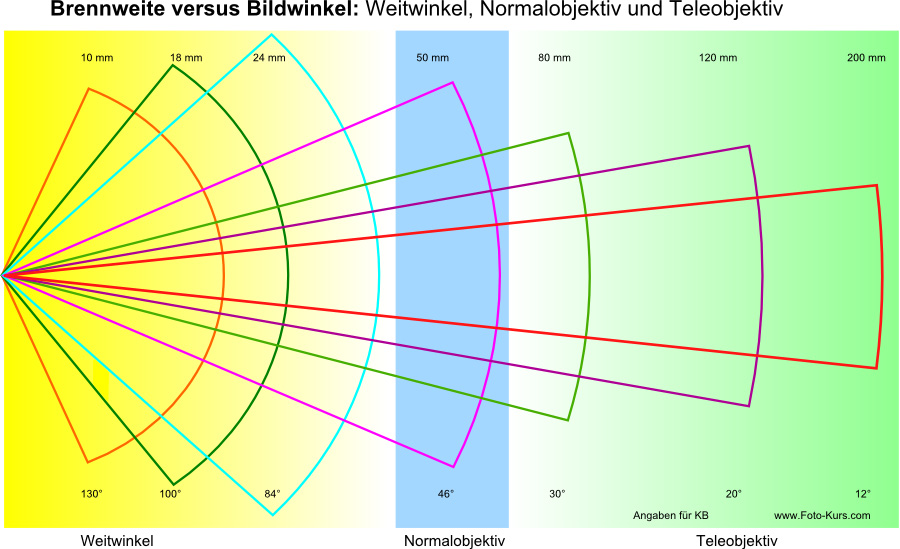
\includegraphics[width=0.7\textwidth]{abb1} 
	\caption[Brennweite und Bildwinkel]{Brennweite und Bildwinkel\footnotemark}\label{fig:abb1}
\end{figure}
\footnotetext{Quelle: https://www.foto-kurs.com/objektiv-digitalkamera.htm}
\begin{itemize}
	\item Normalobjektiv
		\begin{itemize}
		\item Das Normalobjektiv entspricht im Grunde dem menschlichen Blickwinkel, und wird meist als natürlich empfunden.\citep{normalobjektiv}
		\end{itemize}
	\item Weitwinkel
		\begin{itemize}
		\item Wie man auf der obigen Abbildung sehen kann, haben Weitwinkelobjektive einen breiten Bildwinkel, somit sieht man mehr vom Bild.\citep{normalobjektiv}
		\end{itemize}
	\item Teleobjektiv
		\begin{itemize}
		\item Teleobjektive nehmen Objekte mit einem kleinen Blickwinkel aus großer Entfernung auf. Teleobjektive haben daher einen eher kleinen Schärfentiefenbereich, was sich beispielsweise für Interviews schlecht eignet.\citep{tele}
\end{itemize}
\end{itemize}
\paragraph{Schärfentiefe}
\leavevmode \\
"Die Schärfentiefe ist das Maß für den in einem Bild scharf abgebildeten Bereich." (Jörg Jovy, 2017, S. 223)\newline
Der Sinn der Schärfentiefe ist, ein Objekt oder Motiv vom Hintergrund abzuheben, also es schärfer darstellen zu lassen als den Hintergrund.\citep{scharf}\newline
Die Schärfentiefe kann durch drei Parameter eingestellt werden:
\begin{itemize}
	\item Sensorgröße
	\item Blende
	\item Brennweite
\end{itemize}
Wie vorhin erklärt, hat der Sensor auch einen Einfluss auf die Schärfentiefe, nämlich je größer der Sensor ist, desto mehr Spielraum bietet sich.\newline
Je weiter die Blende geöffnet ist, desto geringer ist die Schärfentiefe. Zuletzt kann noch die Brennweite eingesetzt werden, um eine geringe Schärfentiefe zu erzeugen. Je näher man an ein Objekt heranzoomt, desto unschärfer wird der Hintergrund.\citep{scharfZwei}\newline 
Bei allen drei Videos wurden Zoomobjektive verwendet. Zoomobjektive haben eine variable Brennweite, das heißt man muss sich nicht auf eine fixe Brennweite festlegen, sondern kann selbst entscheiden welche Brennweite man haben möchte. Bei dem Dreh der Videos kam das Canon Objektiv EF-S 18-135mm f/3.5-5.6 IS USM zum Einsatz. Durch das Zoomobjektiv war es möglich das Filmen flexibel zu gestalten.\newline
Beim Dreh des Interviews mit dem Abteilungsvorstand wurde die Brennweite nicht berücksichtigt und somit hat die nötige Schärfentiefe im Bild gefehlt. Dies wurde anschließend in der Post Production nachträglich nachbearbeitet. Bei dem Tag der offenen Tür Video konnte mit dem Wissen, dass die Brennweite auch einen Einfluss auf die Schärfentiefe hat, die optimale Schärfentiefe erzielt werden.
\section[Beleuchtung]{Beleuchtung\protect\footnote{\label{}vgl. Jörg Jovy, 2017, S. 236ff.}}
In der Videografie wird die Belichtungszeit in der Bildrate vorgegeben, wohingegen sie in der Fotografie zwischen mehreren Stunden und wenigen Sekunden liegen kann.
Die richtige Belichtungszeit kann man sich mit folgender Formel berechnen: Belichtungszeit = 1: Framerate x 2. Nimmt man nun mit 25 Bildern pro Sekunde auf, ergibt sich eine Belichtungszeit von 1:50 = 1/50 s. Würde man die Belichtungszeit verkürzen, z.B. auf 1/125 s, dann würde das Bild zwar schärfer werden, aber dann würde die Gefahr bestehen, dass der sogenannte Moir\'{e} Effekt eintritt. Der Moir\'{e} Effekt ist ein Bildfehler, der bei bewegten Bildern ein Flimmern erzeugt. Bei dem "Effekt" liegen feine Muster oder Raster in einem gegeneinander verschobenen Winkel übereinander, welche sich gegenseitig beeinflussen. 
\begin{figure}[H]
	\centering
	
\includegraphics[width=0.8\textwidth]{abb2} 
	\caption{Moir\'{e}-Effekt}
\end{figure}
Bei der Beleuchtung muss man drei Positionen von den Lichtquellen der Belichtung unterscheiden. Das Licht, das von vorne auf den Gegenstand kommt, nennt man Gegenlicht. Das Licht, das von der Seite kommt, wird als Streiflicht bezeichnet, und als drittes Licht wird das Auflicht verwendet, welches von hinten auf das Objekt scheint.
\begin{figure}[H]
	\centering
	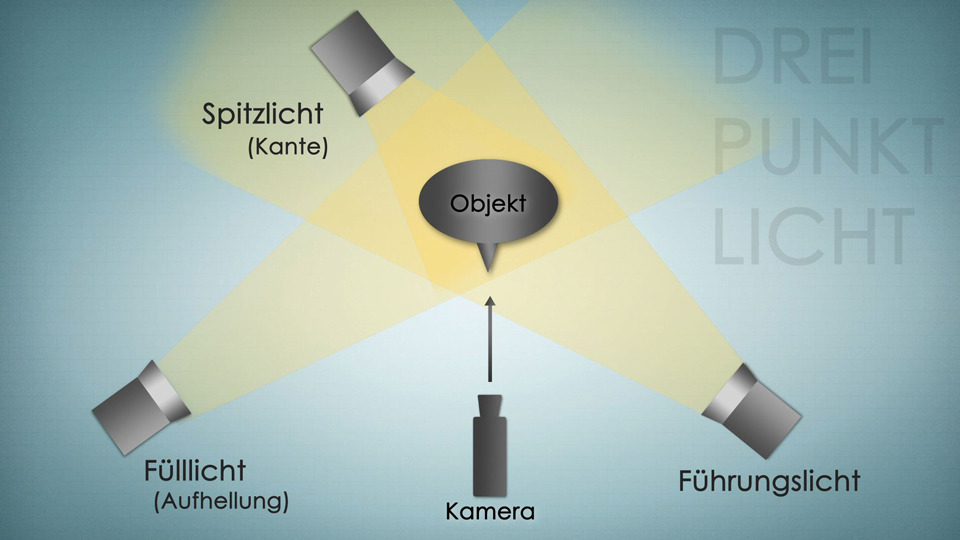
\includegraphics[width=0.7\textwidth]{abb3} 
	\caption{Zusammenspiel der Lichter}\label{fig:abb3}
\end{figure}
Wie man auf der Abbildung \ref{fig:abb3} erkennen kann, ist es wichtig, wie die Lichter im Verhältnis zueinander stehen. Das Führungslicht, oder auch Hauptlicht genannt, dient dazu, die Szene generell aufzuhellen. Durch die Verwendung des Führungslichts entstehen Schatten, die wiederrum mit dem Fülllicht reduziert werden. Um den Gegenstand auch optisch vom Hintergrund abzuheben, kommt das sogenannte Spitzlicht zum Einsatz. \footnote{\label{}vgl. http://www.filmmachen.de/tipps-und-tricks/licht/3-punkt-beleuchtung [Zugriff: 17.03.2018]}
\paragraph{Softbox}
\leavevmode \\
Um den Schauplatz genügend auszuleuchten, verwendeten wir für alle vier Videos LED Scheinwerfer. Um keine harten Schatten zu erzeugen, wurden noch zusätzlich Softboxen verwendet. Eine Softbox ist im Grunde eine Hülle, bei der
die Innenseite silber ist und welche dadurch das Licht wie ein Reflektor nach vorne reflektiert. Anschließend geht das Licht durch den "Front - Diffuser", was
ein lichtdurchlässiges Gewebe ist, der das Licht streut, und es so diffuser erscheinen lässt. Dadurch wird auch die Helligkeit reduziert und aufgrund der großen Fläche wird das Licht weicher, wodurch die Schatten diffuser werden. \newline
Bei dem Interview mit dem Abteilungsvorstand wurde jedoch keine 3-Punkt-Beleuchtung angewandt. Es wurde nur mit zwei Lichtquellen gearbeitet, um kein gekünsteltes Video zu erstellen. Die zwei Lichtquellen sollen nur dazu dienen, die Szene generell aufzuhellen und, um eventuelle Schatten auszugleichen. Es soll natürlich wirken und dem Betrachter nicht das Gefühl geben, dass es gestellt ist.  Dieses Set wurde ebenfalls bei dem Dreh des Quiz mit dem Absolventen und dem Schüler der zweiten Klasse angewandt, um auch hier ein natürliches Ergebnis zu erzeugen.
\section{Mikrofone}
\subsection{Richtcharakteristik}
\begin{quote}
"Die Richtcharakteristik definiert, aus welcher Richtung das Mikrofon den Schall besonders empfindlich aufnimmt. Stark vereinfacht gesagt: Aus welcher Richtung aufgenommen wird." (https://www.delamar.de/mikrofon/richtcharakteristik-mikrofon-22647/ [Zugriff: 17.03.2018])
\end{quote}
\subsubsection{Kugelcharakteristik}
Bei der Kugelcharakteristik wird der Schall von allen Richtungen aufgenommen, das heißt es wird von keiner bevorzugten Richtung aufgenommen. Das Problem, was dadurch entsteht, ist, dass die Rückkoppelanfälligkeit sehr hoch ist, wodurch Mikrofone mit einer Kugelcharakteristik schlecht für Bühnen geeignet sind.\citep{kugel}
\begin{figure}[H]
	\centering
	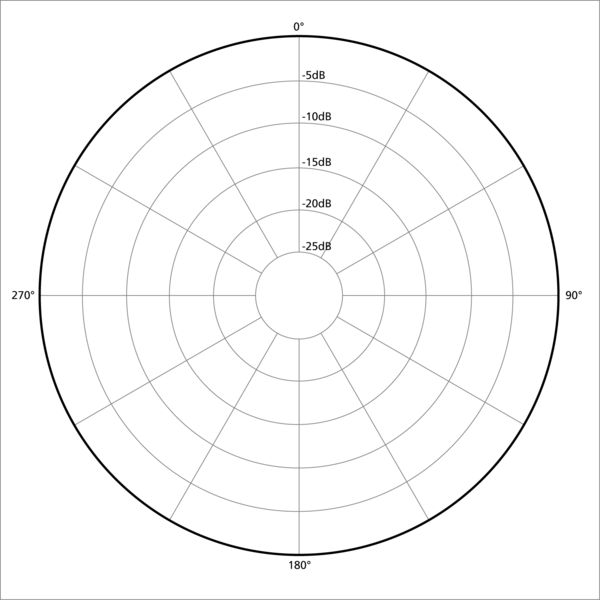
\includegraphics[width=0.4\textwidth]{abb4} 
	\caption[Kugel]{Kugel\footnotemark}
\end{figure}
\footnotetext{Quelle: https://www.delamar.de/mikrofon/richtcharakteristik-mikrofon-22647/}
\subsubsection{Nierencharakteristik}
Die Niere nimmt, im Gegensatz zur Kugelcharakteristik, aus einer bevorzugten Richtung auf. Im Gegensatz zu der Kugelcharakteristik, bei der der Schall von allen Seiten aufgenommen wird, wird er bei der Niere nur von einer Seite aufgenommen, meistens von vorne. Der Schall wird von den Seiten nur sehr leise bis gar nicht aufgenommen. Der Vorteil der Niere ist, dass sie rückkopplungsfester, als die Kugel ist und sie so auch beispielsweise bei Konzerten verwendet werden kann. Der Nachteil der Niere ist der sogenannte Nachbesprechungseffekt.\citep{naheffekt}\citep{kugel} Das bedeutet: "Ab einer gewissen Nähe der Schallquelle werden die tieffrequenten Anteile dominanter." (https://www.delamar.de/faq/nahbesprechungseffekt-34021/ [Zugriff: 17.03.2018])
\begin{figure}[H]
	\centering
	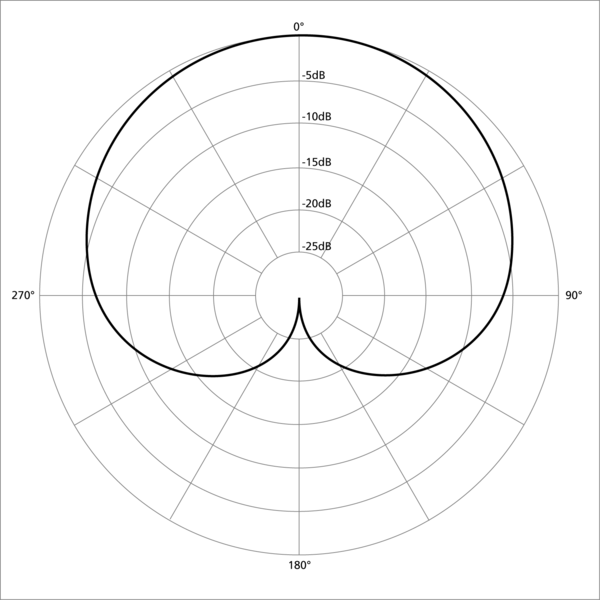
\includegraphics[width=0.4\textwidth]{abb5} 
	\caption[Niere]{Niere\footnotemark}
\end{figure}
\footnotetext{Quelle: https://www.delamar.de/mikrofon/richtcharakteristik-mikrofon-22647/}
\subsubsection{Keule/Superniere}
Keule beziehungsweise Superniere sind Charakteristiken, die von der Niere abgeleitet sind. Die Fläche der Keule ist im Gegensatz zu der Niere etwas schmaler. Das hat die Auswirkung, das von den Seiten weniger aufgenommen wird. Dadurch sind Mikrofone mit einer Keule oder Superniere hinten empfindlicher.\citep{kugel} "Dennoch haben sie die höchste Rückkopplungsfestigkeit." (https://www.delamar.de/mikrofon/richtcharakteristik-mikrofon-22647/ [Zugriff: 17.03.2018])
\begin{figure}[H]
	\centering
	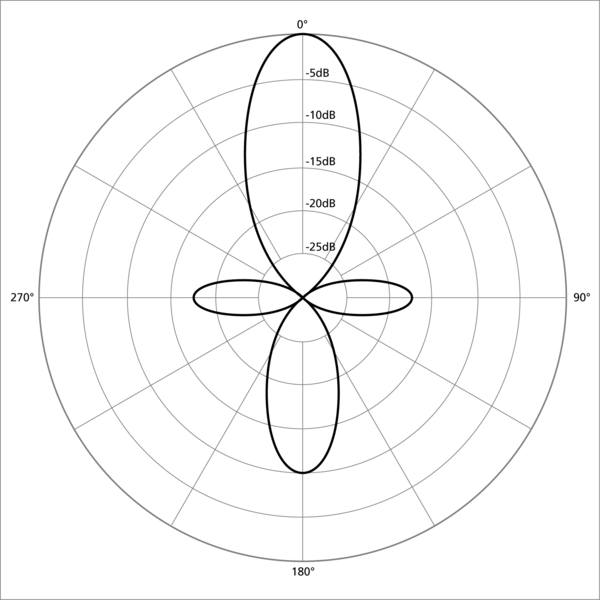
\includegraphics[width=0.4\textwidth]{abb6} 
	\caption[Keule]{Keule\footnotemark}
\end{figure}
\footnotetext{Quelle: https://www.delamar.de/mikrofon/richtcharakteristik-mikrofon-22647/}
\subsubsection{Acht}
Die sogenannte Achtcharakteristik nimmt den Schall von vorne und hinten auf, jedoch nur minimal von den Seiten. Diese Charakteristik hat die Verwendung bei der M/S-Stereofonie.\citep{kugel}\newline
Bei der M/S-Stereofonie, oder auch Mid/Side-Stereofonie, werden die Audiosignale mittig und von der Seite aufgenommen. In der Mitte befindet sich ein Mikrofon mit einer Nierencharakteristik, wohingegen die Seitensignale mit einer Achtcharakteristik aufgenommen werden. Die Seitensignale nehmen die Schallquellen aus unterschiedlichen Richtungen auf und sind so mit einem menschlichen Ohr zu vergleichen.\citep{ms}
\begin{figure}[H]
	\centering
	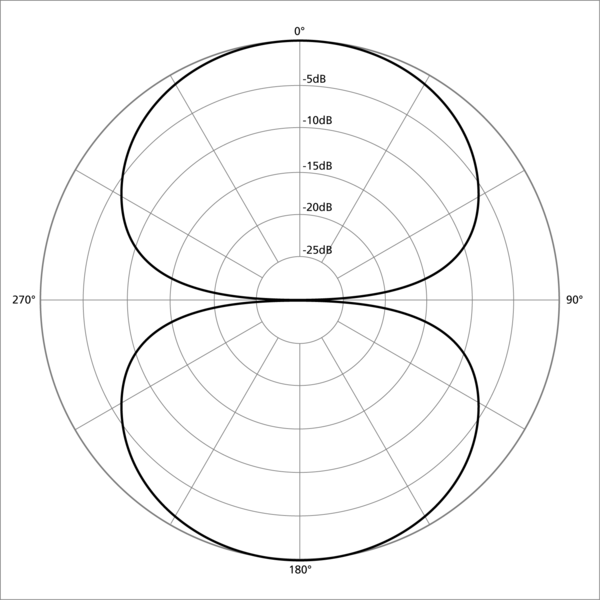
\includegraphics[width=0.4\textwidth]{abb7} 
	\caption[Acht]{Acht\footnotemark}
\end{figure}
\footnotetext{Quelle: https://www.delamar.de/mikrofon/richtcharakteristik-mikrofon-22647/}
\subsection{Kondensatormikrofon}
"Ein Kondensatormikrofon wandelt Schall in ein elektrisches Signal." (https://www.delamar.de/faq/kondensatormikrofon-34728/ [Zugriff: 17.03.2018])\newline
Bei einem Kondensatormikrofon treffen die Schallwellen zuerst auf die Membran, was eine leitende Folie ist, die mit Gold bedampft ist. Dies verbessert die  Leitfähigkeit des Mikrofons, was die Luftdruckschwankungen in mechanische Schwingungen umwandelt. Anschließend wird sie in elektrische Spannung umgewandelt und über die XLR-Buchse wieder ausgegeben.\citep{kondensator}
\begin{figure}[H]
	\centering
	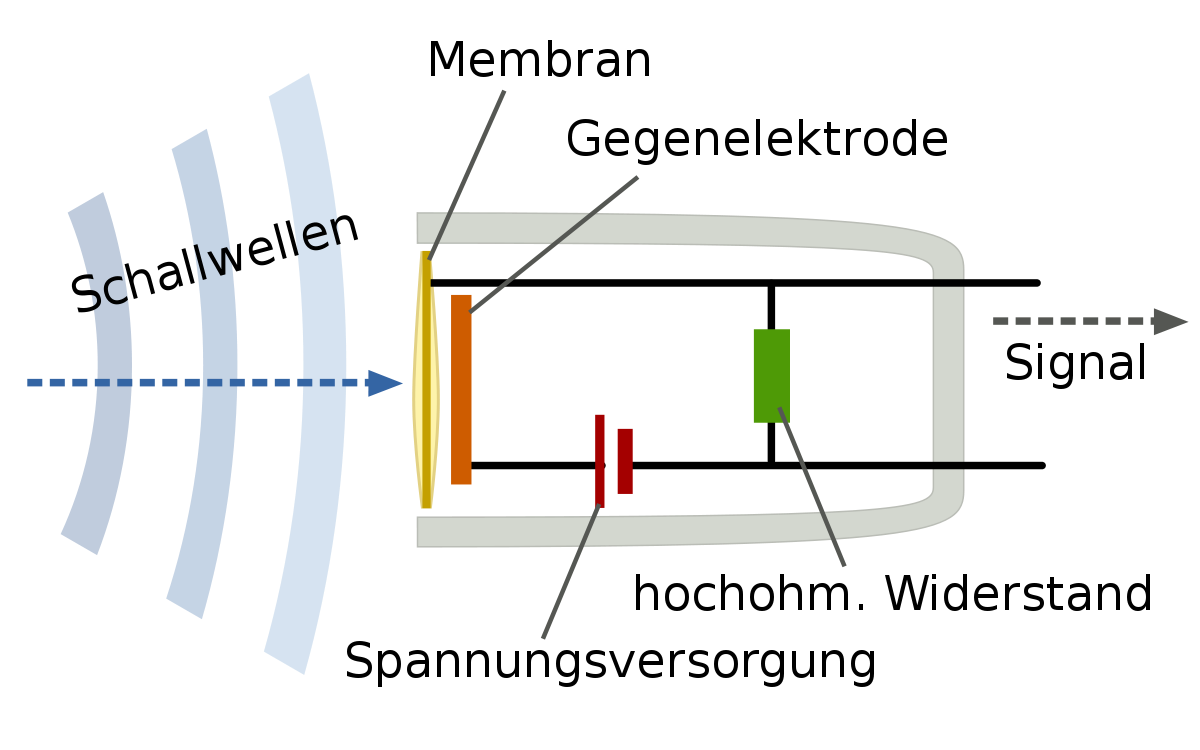
\includegraphics[width=0.6\textwidth]{abb8} 
	\caption[Kondensatormikrofon]{Kondensatormikrofon\footnotemark}
\end{figure}
\footnotetext{Quelle: https://de.wikipedia.org/wiki/Kondensatormikrofon\#/media/File:Kondensatormikrofon.svg}
\subsection{Dynamisches Mikrofon}
\begin{quote}
"Bei diesem Mikrofontyp wird das Signal durch elektromagnetische Induktion erzeugt. Kurz: Der Schall trifft auf die Membran des Mikrofons und regt sie zu mechanischen Schwingungen an, die durch eine mit der Membran verbundene Spule in elektrische Spannung umgewandelt werden. Und diese kommt dann aus der (XLR-)Buchse des Mikrofons." (https://www.delamar.de/faq/dynamisches-mikrofon-34718/ [Zugriff: 17.03.2018])
\end{quote} 
\begin{figure}[H]
	\centering
	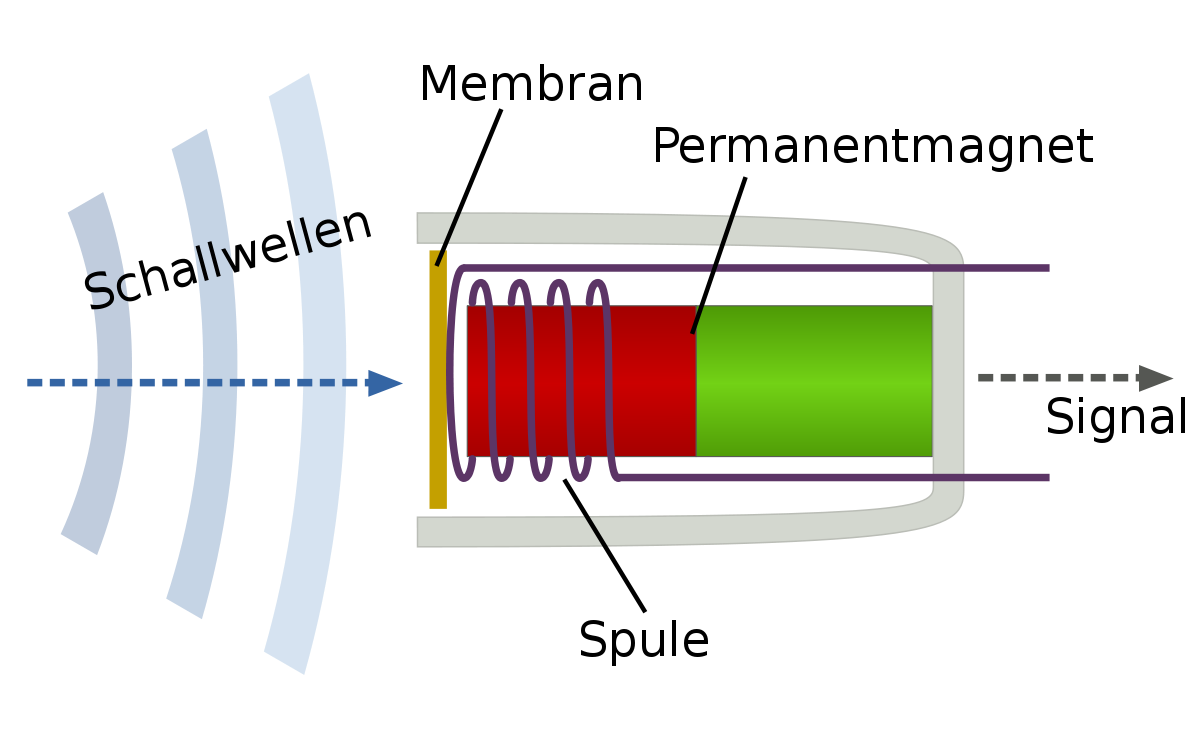
\includegraphics[width=0.6\textwidth]{abb9} 
	\caption[Dynamisches Mikrofon]{Dynamisches Mikrofon\footnotemark}
\end{figure}
\footnotetext{Quelle: https://de.wikipedia.org/wiki/Dynamisches\_Mikrofon\#/media/File:Tauchspulenmikrofon.svg}
\paragraph{Interview mit Abteilungsvorstand}
\leavevmode \\
Bei der Aufnahme des Videos mit dem Abteilungsvorstand Dr. Hager wurde das t-bone GZ 400 Grenzflächen-Mikrofon verwendet. Das Mikrofon arbeitet mit der Richtcharakteristik Superniere. Das Mikrofon wurde in die Mitte des Tisches platziert, um die Stimmen der Interviewerin und des Abteilungsvorstandes einzufangen.\newline
Bei dem Video wurden bewusst keine Ansteckmikrofone verwendet, um nicht das typische Interview-Bild widerzuspiegeln, wo die Mikrofone an den Personen angesteckt werden und man diese dann auch im Video sieht.
\paragraph{Tag der offenen Tür}
\leavevmode \\
Bei dem Tag der offenen Tür Video wurde eine Angel für die Aufnahme der Interessenten verwendet. Hierfür wurde eine Keule beziehungsweise eine Superniere eingesetzt. Dies war deswegen notwendig, da am Tag der offenen Tür viele Hintergrundgeräusche vorhanden waren. Hätte man mit einer Kugelcharakteristik aufgenommen, würde man die Hintergrundgeräusche auch hören, im Gegensatz zu der Keule, welche hauptsächlich von vorne aufnimmt und Hintergrundgeräusche ausblendet.
\paragraph{Video mit einem Absolvent}
\leavevmode \\
Beim Quiz mit dem Absolventen und dem Schüler der zweiten Klasse wurde, wie beim ersten Interview, das Grenzflächen-Mikrofon verwendet.
\section{Planung und Vorbereitung}
Für die Planung eines Videos benötigt man meistens viel Zeit, um auch ein gutes Ergebnis zu erzielen. Bevor es an das bekannte Drehbuch geht, muss man vorerst noch drei andere Schritte berücksichtigen, nämlich die sogenannte Logline, das Expos\'{e} und das Treatment. Erst nach diesen Schritten ist es sinnvoll das Drehbuch zu schreiben.\citep{planung}
\subsection{Logline}
Die Logline ist, vereinfacht gesagt, die Idee zum Film oder zum Video. Die Logline besteht meistens nur aus einem Satz und soll nur einen groben Überblick über den Film oder des Videos preisgeben.\citep{logline}
\begin{figure}[H]
	\centering
	
\includegraphics[width=1.0\textwidth]{abb26} 
	\caption{Logline des Tag der offenen Tür Videos}
\end{figure}
\subsection{Expos\'{e}}
Das Expos\'{e} besteht meist nur aus ein paar Skizzen, wobei folgende Themen behandelt werden: das Thema selbst, die Besonderheiten des Videos oder Films, die Protagonisten, Drehorte und sonstige Herausforderungen. Das Expos\'{e} soll den Mitarbeitern dazu dienen, weitere Entscheidungen leichter zu treffen.\citep{expose}
\subsection{Treatment}
Das Treatment ist mehr oder weniger der Vorgänger des Drehbuchs. Ein Treatment beinhaltet schon kurze Dialoge zu bestimmten Szenen und eine szenengenaue Auflösung zum Film oder zum Video.\citep{treatment}
\subsection{Drehbuch}
Das Drehbuch ist, im Vergleich zum Treatment, komplett ausgearbeitet, das heißt, es liegt ein kompletter Produktionsleitfaden vor, wobei jede Szene ausgearbeitet ist. Weiters werden wichtige Einstellungen in Bildszenen dargestellt. Adobe bietet die kostenlose Software \textit{Story} an, mit der man Drehbücher erstellen kann.\citep{drehbuch}\newline
Story ist eine Software von Abdobe, mit der man Drehbücher erstellen kann. Bei der Erstellung kann man ein vorgefertigtes Template auswählen und anschließend kann man schon das Drehbuch verfassen. Bei der Erstellung des Drehbuchs kann man zwischen Scene Heading, Action, Character, Parenthetical, Dialog, Transition, Speaking Extra, Shot und General auswählen. Diese Elementtypen sind auch schon dementsprechend formatiert und man muss weder etwas einrücken, noch sonstige Formatierungen einstellen.\citep{drehbuchZwei}\\ \\
Da nur Interviews geplant wurden und man bei Interviews keine Szenen planen kann, wurde das Expos\'{e}, das Treatment und das Drehbuch übersprungen. Jedoch wurde eine Logline und das Storyboard verfasst und zusätzlich wurde noch ein Fragenkatalog pro Video erstellt. 
\subsection{Storyboard}
Ein Storyboard ist eine visualisierte Veranschaulichung von dem Konzept, das man sich zuvor überlegt hat.\citep{storyboard} Um die korrekte Ausführung der Videos zu gewährleisten, wurden Storyboards angefertigt. Diese wurden mit der Online Plattform "Storyboard That"\citep{storyboardLink} erstellt und schließlich als PDF - Format exportiert.
Im Storyboard wurden die Szenen bildlich dargestellt, was das Team im weiteren Verlauf unterstützte, da es dadurch grobe Fehler vermeiden konnte.
Das Online - Tool ermöglichte es zwischen verschiedensten Szenen, Charakteren und Kategorien auszuwählen, wodurch vereinfacht, verschiedenste Szenen dargestellt werden konnten. 
\begin{figure}[H]
\begin{center}
	\fbox{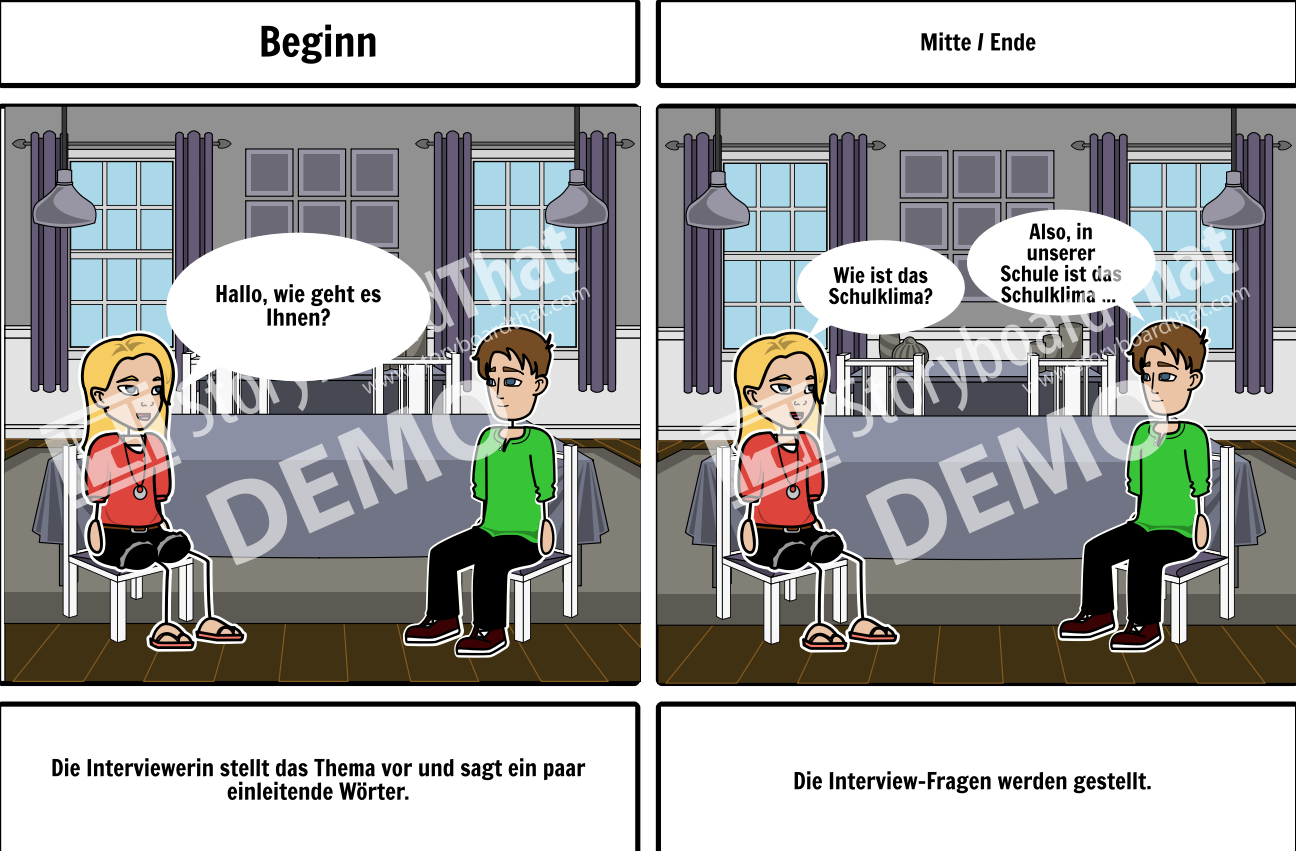
\includegraphics[scale=0.30]{abb10}}
	\caption{Storyboard des Interviews mit dem Abteilungsvorstand}
\end{center}
\end{figure}
\section{Setting}
Beim Aufbau des Sets wurde auf das Drehbuch und das Storyboard referenziert. Hierbei wurde auch die Location berücksichtigt, da für den Aufbau eines Videos mit Greenscreen ein anderes Set von Nöten war, als bei einem Video am Gang in der Schule. Weiters musste überlegt werden, wie die Kameras und Lichter platziert werden müssen. Bevor es zum eigentlichen Dreh kam, wurde das Setting im Vorhinein ausreichend getestet, um später beim wirklichen Dreh, Fehler zu vermeiden. Weiters wurden zusätzlich verschiedene Mikrofone getestet, um für die jeweilige Situation das optimale Mikrofon zu verwenden.
\section{Post Production}
\subsection{Aufnahmeformate}
Bei der Auswahl des Aufnahmeformates muss man sich im Klaren sein, mit welchem Codec man aufnehmen möchte. Hierbei muss man zwischen Codecs und Containern unterscheiden. Container, welche den Videostream mittels eines Codecs digitalisieren, speichern die Videodaten auf dem Speicherchip. Audio Video Interleave (AVI), QuickTime (MOV) oder Moving Pictures Expert Groups (MPEG) sind zum Beispiel solche Containerformate. Ein Codec wandelt analoge Bilder in digitale Datenströme um. Bei der Codierung wird das Bild komprimiert, was wiederum mehr Speicherplatz zur Verfügung stellt. DivX, QuickTime H.264, Apple ProRes, Panasonic AVC-Intra oder Avid DNxHD sind typische Codecs.\footnote{vgl. Jörg Jovy, 2017, S. 114f.}\newline
Die Komprimierung des Videosignals erfolgte bei allen vier Videos mittels dem H.264 Codec im QuickTime (MOV) Container. 
\paragraph{MPEG}
\leavevmode \\
"MPEG ist ein standardisiertes Kompressionsverfahren, das sich speziell zur Datenreduktion von Bewegtbildern eignet." (https://www.film-tv-video.de/term-word/mpeg/ [Zugriff: 26.03.2018]) MPEG lässt dem Gerätehersteller freie Wahl, bezüglich der Entscheidung der Datenerzeugung. Jedoch legt MPEG das Datenformat und die Dekodierung vor. Was noch beachtet werden muss, ist, dass schlussendlich ein normgerechter MPEG-kodierter Datenstrom entstehen muss, der mit einem MPEG-Decoder gelesen und wiedergegeben werden kann. Bei dem MPEG Standard setzen sich die Einzelbilder einer Videosequenz aus einer Folge von I-, B- und P-Frames zusammen. Diese Aufeinanderfolgung wird Group of Pictures, kurz GOP, genannt. Eine Group of Pictures muss mindestens ein I-Frame enthalten. I-Frames sind Indexbilder, welche die wichtigsten Bildinformationen enthalten. "B-Frames sind  bidirektionale Bilder, also Frames, die nur die Unterschiede eines Bildes zum vorhergehenden oder folgenden Bild beinhalten." (https://www.film-tv-video.de/term-word/mpeg/ [Zugriff: 26.03.2018]) P-Frames sind Predicted Frames. Predicted Frames werden aus den vorherigen I-Frames berechnet.\newline
\begin{figure}[H]
	\centering
	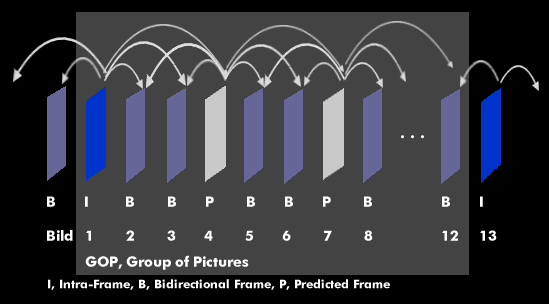
\includegraphics[width=0.8\textwidth]{abb27} 
	\caption{Group of Pictures}
\end{figure}
Der QuickTime Container ist im Grunde, wie das MPEG Containerformat aufgebaut. Jedoch ist QuickTime ein eigenes Containerformat von Apple.\footnote{vgl. https://www.film-tv-video.de/term-word/mpeg/ [Zugriff: 26.03.2018]}
\subsection{Kompressionsverfahren}
Bei der Bildkompression werden die Bildinformationen in 4x4, 8x8 oder 16x16 Pixeln zusammengefasst. "In einzelnen Bildern und zwischen aufeinanderfolgenden Bildern werden dann sich wiederholende Daten identifiziert." (Jörg Jovy, 2017, S. 117)\newline
Nun können die wiederholenden Informationen gefiltert und weggelassen werden. Bei dem MPEG-2 Container wird zum Beispiel nur jedes zwölfte Bild komplett gespeichert, wobei bei den anderen Bildern nur Teile beziehungsweise Veränderungen gespeichert werden. Da nur jedes zwölfte Bild komplett gespeichert wird, ist das Risiko enorm groß, dass Artefakte, also Bildfehler, entstehen können. Die sogenannten Artefakte entstehen bei der Umwandlung von digitalen Bildern in analoge Bildsignale.\footnote{vgl. Jörg Jovy, 2017, S. 117}
\subsection{Schnittprogramme}
\paragraph{Lightworks}
\leavevmode \\
Lightworks ist ein lizenzfreies Videoschnittprogramm, das auf Windows, Linux und auf IOS Betriebssystemen verwendet werden kann. Lightworks bietet nicht nur die freie Version, sondern auch eine Pro Version. Die freie Version bietet dem User eine Vielzahl an importierbaren Formaten, wie zum Beispiel Apple Pro Res, AVC-Intra 50, MPEG-2 Long GOP und vieles mehr. Weiters kann man in Lightworks seine Videos mit dem Codec H.264 mit der Auflösung 1280x720p kodieren.\footnote{vgl. Jörg Jovy, 2017, S. 355}\footnote{vgl. https://www.lwks.com/index.php?option\=com\_content\&view\=article\&id\=102\&Itemid\=213 [Zugriff: 02.04.2018]}
\paragraph{Adobe Premiere Pro}
\leavevmode \\
Adobe Premiere Pro ist eine kostenpflichtige Software, welche aber eine Vielzahl von Funktionalitäten bietet. Im Gegensatz zu Lightworks bietet Adobe Premiere Pro eine freie Auswahl, welche Formate man importieren möchte. Weiters bietet Premiere Pro eine umfangreiche Dokumentation. Zusätzlich sind Adobe Programme ähnlich aufgebaut und sind so einfach miteinander zu verknüpfen, wie zum Beispiel Premiere Pro mit Adobe After Effects.\footnote{vgl. Jörg Jovy, 2017, S. 358f.}
\subsection{Schnitt}
Bevor mit dem Schnitt begonnen werden kann, muss zunächst das Projektformat festgelegt werden. Bei Erstellung einer neuen Sequenz können folgende Parameter eingestellt werden
\begin{itemize}
	\item Bilder pro Sekunde
	\item Pixel - Seitenverhältnis
	\item Audio-Samplerate
	\item Bildgröße in Pixeln
	\item Render-Qualität
\end{itemize}
Hat man diese Eigenschaften festgelegt, kann man auch schon mit dem Schnitt beginnen. Es gibt drei Arten des Filmschnitts. Den Rough Cut oder schnelle Schnitt, 3-Punkt-Schnitt oder der exakte Schnitt und den 4-Punkt-Schnitt oder Zeitinterpolation.\footnote{vgl. Jörg Jovy, 2017, S. 384ff., S. 422ff.}
\subsection{Blenden}
Blenden signalisieren dem Zuschauer, dass es sich um eine neue Szene handelt. Blenden sind ein wertvolles Mittel, um den Film oder das Video angenehmer zum Ansehen machen. In Adobe Premiere gibt es eine Vielzahl an unterschiedlichen Blenden, bei denen man sich vorher überlegen sollte, was man mit der Blende bewirken will. In Premiere gibt es nicht nur typische Blenden, wie "Weiche Blende" oder "Filmblende", sondern auch Effektblenden. Die meisten Effektblenden werden jedoch nicht eingesetzt, da sie den Zuschauer nicht besonders ansprechen. Die einzige Effektblende, die verwendet wird, ist die Wipe oder auch Schiebeblende genannt.\footnote{vgl. Jörg Jovy, 2017, S. 438ff.}\newline
Bei dem Schnitt des Tag der offenen Tür Videos kam eine Blende zum Einsatz, nämlich die "Weiche Blende". Die weiche Blende wurde für die Übergänge verwendet von einer Frage zu der Antwort oder zum Ausblenden eines Textes.\newline
Bei dem Schnitt des Videos mit dem Absolventen kamen drei verschiedene Blenden zum Einsatz:
\begin{itemize}
	\item Wegschieben
	\item Filmblende
	\item Einzoomen \& Auszoomen
\end{itemize}
Die Wegschieben Blende ist sozusagen die Hauptblende und dient dazu, von einer einer Szene zur nächsten überzugehen. Die Filmblende blendet die erzielten Punkte ein und die Ein- und Auszommen Blende wurde für das Einblenden der Antworten genutzt.
\subsection{Color Correction}
Mithilfe der Lumetri-Scopes und der Farbkorrektur in Premiere Pro kann man die Farbe im Bild korrigieren. Einerseits gibt es die Lumetri-Scopes, bei denen man auf einen Blick erkennen kann, welche Farbinformationen nicht so dominant sind, ob das Bild über- oder unterbelichtet ist und wie die Helligkeitsverteilung im Bild ist. Und zum anderen gibt es die Farbkorrektur "Lumetri-Farbe" mit der man die oben genannten Eigenschaften verbessern kann.\footnote{vgl. Jörg Jovy, 2017, S. 520ff.}
\paragraph{Vektorskop}
\leavevmode \\
"Das Vektorskop gibt Auskunft über die Farbverteilung im Bild." (Jörg Jovy, 2017, S. 523) Auf dem Vektorskop sind die Grundfarben aus dem RGB und dem CMYK Farbraum abgebildet. Also: Rot, Grün, Blau, Cyan, Magenta, Yellow. Je weiter der Signalpunkt sich vom Zentrum entfernt, desto höher ist die jeweilige Farbsättigung. Hätte man ein Schwarz-Weiß-Bild würde man einen Punkt in der Mitte sehen.\footnote{vgl. Jörg Jovy, 2017, S. 523}\newline
Wie man auf der Abbildung \ref{fig:abb22} sehen kann, hat das Bild eine hohe Farbsättigung von Yellow und Rot, wohingegen es nur wenige Blauanteile hat.
\begin{figure}[H]
	\centering
	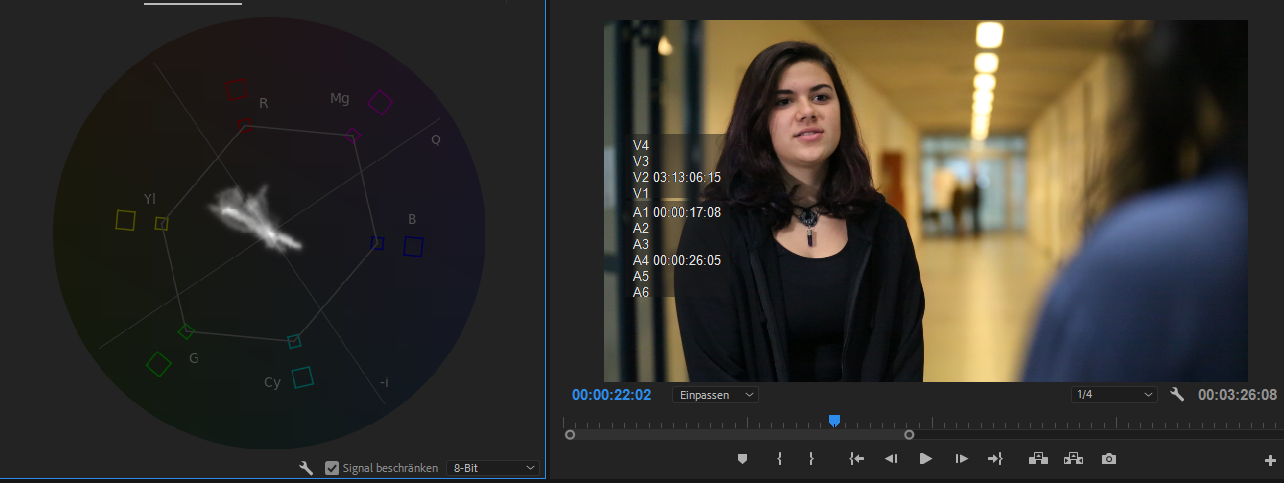
\includegraphics[width=1.0\textwidth]{abb22} 
	\caption{Vektorskop}\label{fig:abb22}
\end{figure}
\paragraph{Histogramm}
\leavevmode \\
Das Histogramm zeigt die Häufigkeitsverteilung von Helligkeit und Farbe, die im Bild vorkommt. Weiters zeigt das Histogramm, ob das Bild korrekt belichtet wurde. Das Histogramm geht von 0,0,0 für RGB Schwarz bis 255,255,255 für RGB Weiß. Die Schatten befinden sich beim Histogramm unten, also in Richtung 0,0,0, wobei man die Lichter oben, also in Richtung 255,255,255 findet.\footnote{vgl. Jörg Jovy, 2017, S. 523f.}\newline
Bei dem Histogramm sieht man, wie bei dem Vektorskop, dass die Farben Yellow und Rot eindeutig dominieren. 
\begin{figure}[H]
	\centering
	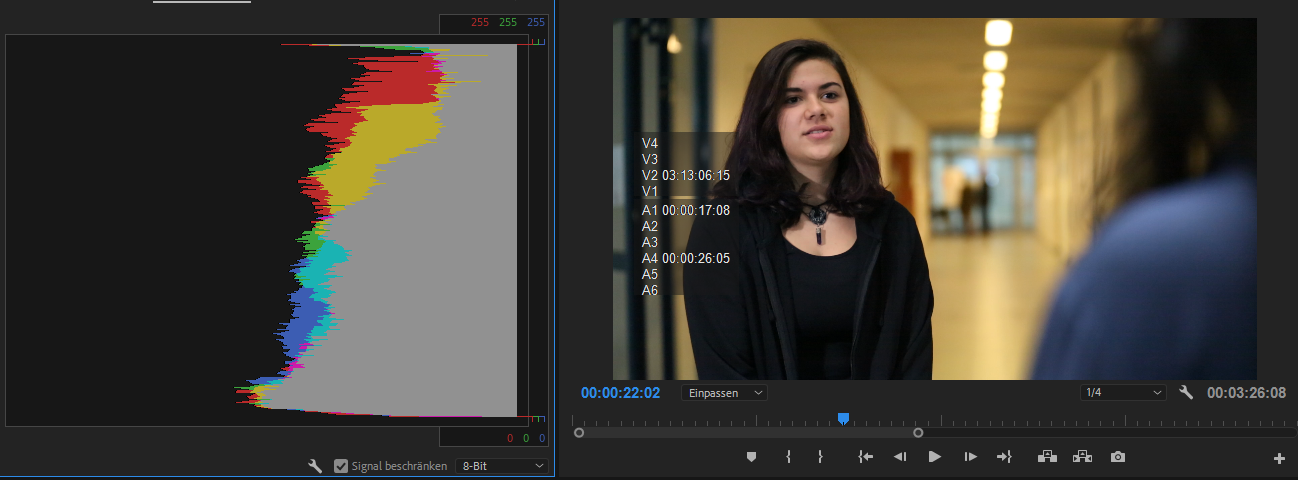
\includegraphics[width=1.0\textwidth]{abb21} 
	\caption{Histogramm}
\end{figure}
\paragraph{Waveform-Monitor}
\leavevmode \\
Der Waveform-Monitor zeigt die Helligkeitsverteilung im Bild. Die Helligkeit wird als Häufigkeitsverteilung wiedergegeben, wobei 100\% Weiß einen Messwert von 100 IRE entsprechen. "IRE ist die international übliche Skalierung." (Jörg Jovy, 2017, S. 522)\newline
0 IRE entsprechen daher Schwarz. Mithilfe des Waveform-Monitors kann man die sogenannten Lichter, Mitten und Tiefen einfach analysieren.\footnote{vgl. Jörg Jovy, 2017, S. 522ff.}\newline
Wie man auf der Abbildung \ref{fig:abb20} sehen kann, reichen die Tiefen bis zu dem Null Wert, das heißt es werden auch die Schatten völlig ausgeschöpft. Die Mitten sollten zwischen 50 und 70\% liegen und befinden sich auch, wie man hier sehen kann, in dem Bereich.\footnote{vgl. Jörg Jovy, 2017, S. 525}
\begin{figure}[H]
	\centering
	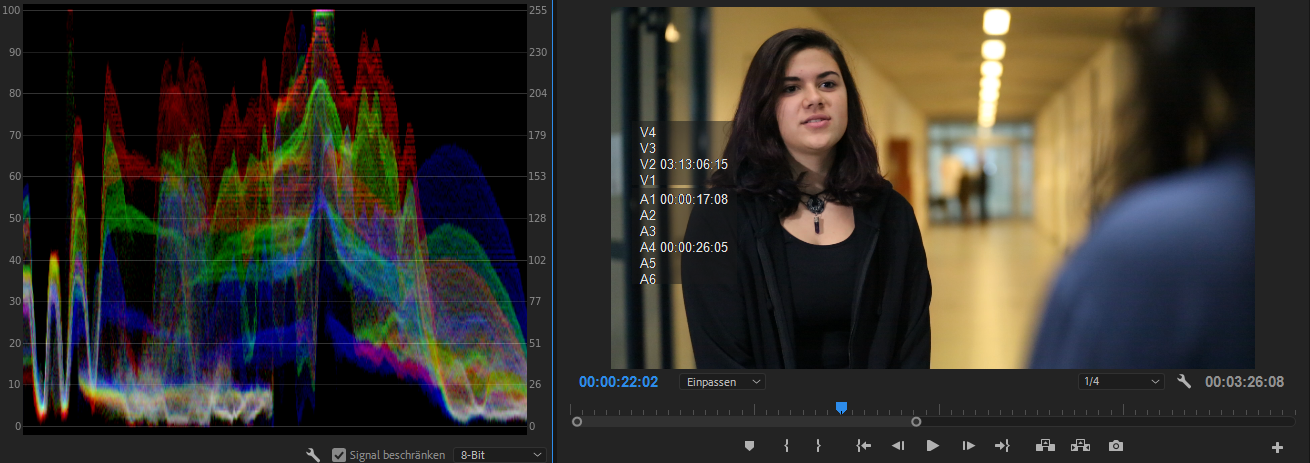
\includegraphics[width=1.0\textwidth]{abb20} 
	\caption{Waveform-Monitor}\label{fig:abb20}
\end{figure}
\subsection{Lumetri-Farbkorrektur}
\paragraph{Einfache Korrektur}
\leavevmode \\
Bei der einfachen Korrektur können grundlegende Verbesserungen vorgenommen werden:\footnote{vgl. https://helpx.adobe.com/at/premiere-pro/using/color-workflows.html [Zugriff: 31.03.2018]}
\begin{itemize}
	\item Weißabgleich
	\item Farbton
	\item Sättigung
\end{itemize}
\paragraph{Kreativ}
\leavevmode \\
Im Kreativ-Bereich kann dem Video ein bestimmter Look verpasst werden, wie zum Beispiel ein CineSpace Look. Weiters kann der Scharfzeichner, die Dynamik und die Sättigung eingestellt werden.\footnote{vgl. https://helpx.adobe.com/at/premiere-pro/using/color-workflows.html [Zugriff: 31.03.2018]}
\paragraph{Kurven}
\leavevmode \\
Bei den Kurven kann man zwischen RGB-Kurven und Farbtonsättigungskurven unterscheiden.\newline
Mit den RGB-Kurven kann die Luminanz und die Farbtonbereiche des Bildes angepasst werden. Man kann die Kurve entweder für alle drei RGB-Kanäle gleichzeitig anpassen, oder man kann es auch für die einzelnen RGB-Farbkanäle anpassen, also für Rot, Grün und Blau.\newline
Bei der Farbtonsättigungskurve kann die Sättigung angepasst werden. Man kann die Sättigung bestimmter Farbtöne verringern und erhöhen.\footnote{vgl. https://helpx.adobe.com/at/premiere-pro/using/color-workflows.html [Zugriff: 31.03.2018]}\newline
Wie man anhand der Abbildung \ref{fig:abb19} sehen kann, ist, dass die rote Farbtonsättigung erhöht wurde. Dies hatte diesen Effekt, dass die Gesichtsfarbe der Person in einen rötlicheren Farbton veränderte.
\begin{figure}[H]
	\centering
	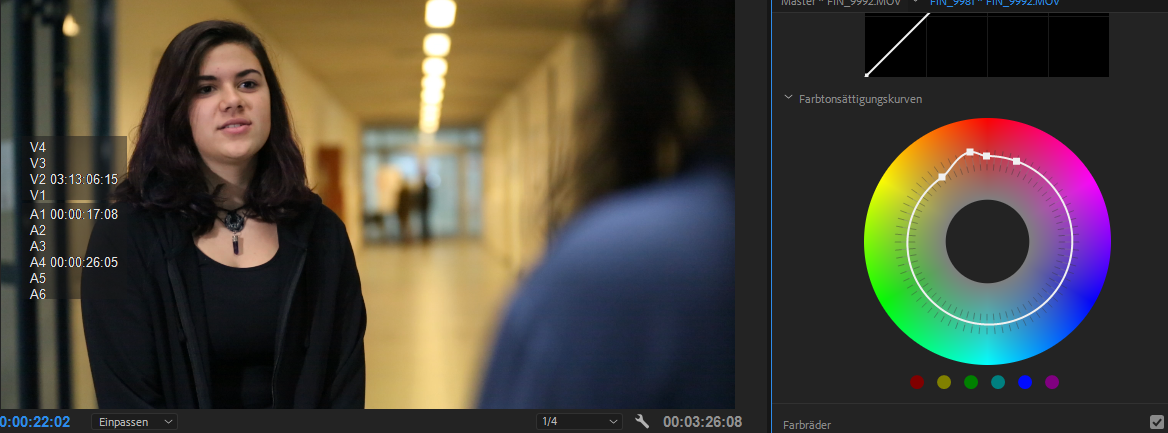
\includegraphics[width=1.0\textwidth]{abb19} 
	\caption{Farbtonsättigungskurve}\label{fig:abb19}
\end{figure}
\paragraph{Farbräder}
\leavevmode \\
Bei den Farbrädern können die Schatten, Mitteltöne und Glanzlichter angepasst werden.\footnote{vgl. https://helpx.adobe.com/at/premiere-pro/using/color-workflows.html [Zugriff: 31.03.2018]}
\subsection{Masken}
In Adobe Premiere Pro kann man mit Masken einen bestimmten Bereich markieren, den man anschließend verändern möchte. In der folgenden Abbildung \ref{fig:abb28} kann man die Verwendung der Maske von dem Interview mit dem Abteilungsvorstand sehen. 
Hierbei wurde die Maske mit einem Weichzeichner versehen, um den Hintergrund unscharf wirken zu lassen. Die Masken können mit einem Ellipsen-Werkzeug, Rechteck-Werkzeug oder einem Zeichenstift erstellt werden. Für die abgebildete Maske kam der Zeichenstift in Verwendung. Nach dem die Maske gezeichnet wsurde, kann man die Maske frame für frame bewegen. In diesem Fall konnte sich die Maske nicht automatisch mitbewegen, da sich der Hintergrund von der Maske nicht abgehoben hat. Somit musste die Maske manuell nachbearbeitet werden.\newline
Um einen flüssigen Übergang zwischen dem Maskenauswahlrahmen und dem Bereich außerhalb der Auswahl zu erzeugen, kann man eine weiche Kante anwenden.\footnote{vgl. https://helpx.adobe.com/de/premiere-pro/using/masking-tracking.html [Zugriff: 31.03.2018]}\begin{quote}Die weichen Kanten glätten den Maskenauswahlrahmen, sodass die Maske mit dem Bereich außerhalb der Auswahl verschmilzt und ein ästhetisch ansprechendes Ergebnis entsteht." (https://helpx.adobe.com/de/premiere-pro/using/masking-tracking.html [Zugriff: 31.03.2018])\end{quote}
Weiters wurde die Maske bei dem Tag der offenen Tür Video angewandt. Dies war deswegen notwendig, da aufgrund des ständigen Lichtwechsels die Gesichtsfarbe der Personen sich immer änderte. 
\begin{figure}[H]
	\centering
	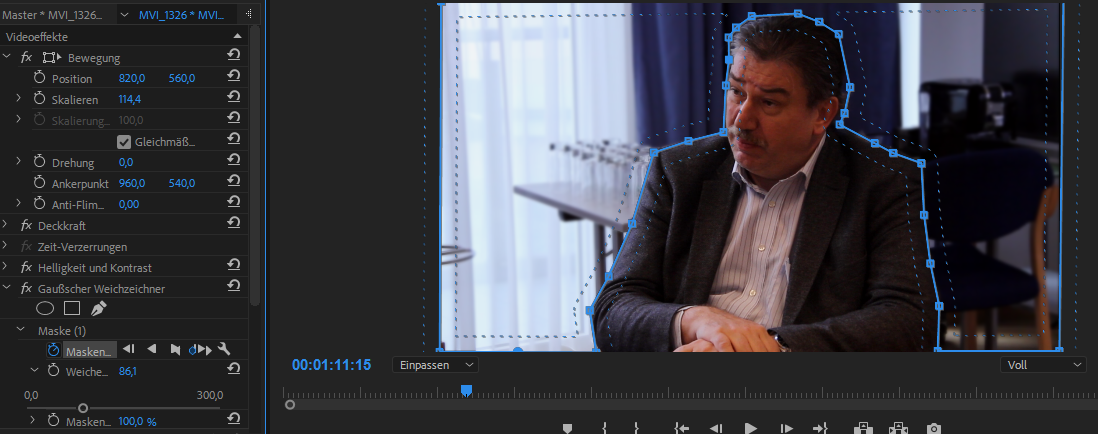
\includegraphics[width=1.0\textwidth]{abb28} 
	\caption{Maskenpfad des Interviews mit dem Abteilungsvorstand}\label{fig:abb28}
\end{figure}
\subsection{Geschwindigkeitseffekte}
Am Tag der offenen Tür wurde der Eingangsbereich der Schule für etwa 20 Minuten gefilmt. Dieses Video wurde schließlich für das Tag der offenen Tür Video verwendet. Um den Zuschauer kein 20 Minuten langes Video anschauen zu lassen, wurde die Geschwindigkeit des Videos beschleunigt, und somit ein Zeitraffer erzeugt. Mit einem Rechtsklick auf die Spur kann man auch schon die Eigenschaft "Geschwindigkeit/Dauer" auswählen, bei der man die Geschwindigkeit beschleunigen oder verlangsamen kann.\footnote{vgl. Jörg Jovy, 2017, S. 475ff.}
\subsection{Musik}
Bei dem Tag der offenen Tür Video und dem Quiz wurde lizenzfreie Musik eingebunden. Diese stammt von Soundcloud. Die Verwendung von Musik lockert das Schauen eines Videos auf und löst beim Menschen Spannung, Mitleid, Angst oder Entspannung aus. Weiters dient die Musik geräuschlose Szenen zu überbrücken und sie so angenehmer machen.\footnote{vgl. Jörg Jovy, 2017, S. 365}
\subsection{Export}
Bei dem Export eines Videos in Adobe Premiere muss man sich zuerst für ein Format entscheiden, in dem man das Video exportieren möchte. Heutzutage wird der H.264 von allen Browsern unterstützt und deswegen wurden auch die Videos in dem Codec kodiert. Jedoch unterstützen veraltete Mozilla Firefox Browser keinen H.264 Codec, sondern den Web.m Codec. Um zu gewährleisten, dass sich jeder User die Videos ansehen kann, wurden die Videos auch im Web.m Codec kodiert. Da Adobe Premiere den Web.m Codec nicht implementiert hat, war es notwendig diesen mittels einer msi Datei einzubinden. \footnote{vgl. https://helgeklein.com/blog/2017/12/browser-video-codecs-formats-hardware-acceleration/ [Zugriff: 02.04.2018]}\footnote{vgl. https://www.soeren-hentzschel.at/firefox/mozilla-integriert-openh264-video-codec-von-cisco-in-firefox-33/ [Zugriff: 02.04.2018]}
\section{Herausforderungen}
\subsection{Interview mit dem Abteilungsvorstand}
Das Problem bei dem Dreh, mit dem Interview des Abteilungsvorstandes, war, dass die Blende zu weit geöffnet war, und so es nicht möglich war die Schärfentiefe zu erzeugen. Die Schärfentiefe wird durch die Blende, der Sensorgröße und der Brennweite definiert. Da man an der Sensorgröße nach dem Kauf der Kamera nichts mehr ändern kann, muss man sich mit den anderen zwei Bereichen auseinandersetzen. Je weiter die Blende geschlossen ist, desto mehr Schärfentiefe kann erzielt werden. Je offener die Blende ist, umso weniger Schärfentiefe hat man. Die Brennweite beeinflusst die Schärfentiefe insofern, da je größer die Brennweite ist, also je näher man an ein Objekt heranzoomt, desto unschärfer wird der Hintergrund. 
Wie man in der Abbildung sehen kann, befinden sich im Hintergrund zu viele Störfaktoren, die aufgrund der fehlenden Schärfentiefe gut erkennbar sind, und dem Zuseher vom eigentlichen Bild ablenken würden. 
Das Programm Adobe Premiere Pro ermöglicht es mittels einer Maske einen Maskenpfad zu setzen, den man später auch "bewegen" kann. Das bedeutet, dass sich die Maske Frame für Frame fortbewegt und sich anpasst. Jedoch war dies hier nur begrenzt möglich, da sich der Hintergrund nicht sonderlich abhebt, und so die Maske sich nicht mitbewegen konnte. Der Maskenpfad musste schließlich bei manchen Frames manuell nachbearbeitet werden.
Man kann beim Erstellen der Maske entscheiden, ob man die Maske mittels einer Ellipsen Form, einer Rechteck Form oder mit einem Zeichenstift erzeugen will. Bevor man die Maske zeichnet, wählt man den Effekt aus, mit dem man arbeiten will. Im folgenden Fall, war es den Hintergrund unscharf zu zeichnen, also war die Verwendung eines Weichzeichners nötig. Man zieht den gewünschten Effekt ins Schnittfenster und anschließend kann man das gewünschte Werkzeug auswählen, in dem Fall den Zeichenstift. Dies war deswegen notwendig, da man auch die Person auswählen musste, was mit einem Kreis oder Rechteck nicht möglich gewesen wäre. Hat man ein Werkzeug ausgewählt, kann man auch schon die Maske setzen. Adobe Premiere Pro bietet zusätzlich noch eine weiche Kante auf Masken anzuwenden. Dies ist deswegen von großer Bedeutung, da ansonsten der maskierte Bereich mit dem anderen nicht "verschmilzen" würde. Das heißt, man würde die harten Kanten zwischen den zwei Objekten deutlich erkennen. Die weiche Kante glättet den Maskenauswahlrahmen und ermöglicht einen schönen Übergang zwischen Maskenkante und dem anderen Bereich.
\subsection{Tag der offenen Tür Video}
Das Video des Tag der offenen Tür wurde am Gang in der Schule gedreht. Da unter anderem manche Lichter immer wieder aus und an gingen, waren oftmals andere Lichtverhältnisse vorhanden. Diese mussten in der Post Production ebenfalls nachbearbeitet werden. Bei der Bearbeitung der Farbe wurden die Lumetri Scopes Grafiken herangezogen. Diese dienten insofern gut, da man auf einen Blick gesehen hat, von welcher Farbe am meisten Information vertreten ist, und wo noch etwaige Farbinformation fehlt. Mithilfe des Vektorskops, Histogramms und des Waveform-Monitors konnte die Farbe korrigiert werden.
\paragraph{Vektorskop}
\leavevmode \\
"Das Vektorskop gibt Auskunft über die Farbverteilung im Bild."\footnote{\label{}buch} Auf dem Vektorskop sind die Grundfarben aus dem RGB und dem CMYK Farbraum abgebildet. Also: Rot, Grün, Blau, Cyan, Magenta, Yellow. Je weiter der Signalpunkt sich vom Zentrum entfernt, desto höher ist die jeweilige Farbsättigung. Hätte man ein Schwarz-Weiß-Bild würde man einen Punkt in der Mitte sehen.
\paragraph{Histogramm}
\leavevmode \\
Das Histogramm zeigt die Häufigkeitsverteilung von Helligkeit und Farbe, die im Bild vorkommt. Weiters zeigt das Histogramm, ob das Bild korrekt belichtet wurde. Das Histogramm geht von 0,0,0 für RGB Schwarz bis 255,255,255 für RGB Weiß. Die Schatten befinden sich beim Histogramm unten, also in Richtung 0,0,0, wobei man die Lichter oben, also in Richtung 255,255,255 findet.
\paragraph{Waveform-Monitor}
\leavevmode \\
Der Waveform-Monitor zeigt die Helligkeitsverteilung im Bild. Die Helligkeit wird als Häufigkeitsverteilung wiedergegeben, wobei 100\% Weiß einen Messwert von 100 IRE entsprechen. "IRE ist die international übliche Skalierung. 0 IRE entsprechen daher Schwarz. Mithilfe des Waveform-Monitors kann man einfach die sogenannten Lichter, Mitten und Tiefen einfach analysieren. 
\subsection{Video mit einem Absolvent}
Da beim Dreh des Videos der Schüler der zweiten Klasse etwas unschärfer war, war es nötig manuell nachzuschärfen. "Mit dem Effekt 'Scharfzeichner' kann der Kontrast an den Stellen mit Farbänderungen verstärkt werden." Jedoch sollte der Effekt sparsam eingesetzt werden, da es schnell unnatürlich wirken kann. Bei dem Video gab es nicht grobe Herausforderungen. Bei dem Video wurden jedoch verstärkt verschiedene Blenden eingesetzt, um es spannend und abwechslungsreich zu gestalten. 
\paragraph{Effektblenden}
\leavevmode \\
Die Effektblende wird als Gestaltungsmittel bezeichnet, mit der man einen Übergang von einem Ereignis zum anderen besser bildlich darstellen kann. Bei dem Quiz mit dem Absolventen und dem Schüler wurde einerseits die Effektblende "Wegschieben", als auch "Einzoomen \& Auszoomen" und "Filmblende" verwendet. Die Blende "Wegschieben" dient dazu von einem Bild,  also zum Beispiel von einer Antwort zur nächsten Frage überzugehen. Der "Einzoomen \& Auszoomen" Effekt wurde beim Einblenden der Antworten verwendet. Zuletzt wurde die "Filmblende" für das Einblenden der Punkte verwendet.


\section{Interview mit einem Fachmann}
\subsection{Idee}
Wir wollten ein Interviewvideo mit einem passionierten Medientechniklehrer drehen, um den Usern unserer Plattform, einen tiefen Einblick in die Medientechnik zu bieten.

\subsection{Ziel}

\subsection{Dreh}

\subsection{Schnitt}

\subsection{Green Screen}

\subsection{Farbkorrektur}



\chapter{Animationsvideo}

\section{Idee}
\renewcommand{\kapitelautor}{Autor: Niklas Kienreich}
Das Animationsvideo sollte als Eyecatcher für die Zielgruppe dienen. Der Gedanke war, Allgemeines über die HTL auf möglichst witzige, ansprechende Weise zu vermitteln. Die Animation schafft das besser, als die restlichen Videos, da man sich bei den Interviews auf eine lockere, aber doch ernste, zielführende Gesprächsführung verlassen hat. Eine Frage die man sich nun aber stellen musste war, wie man das Video animiert. Neben vier Interview Videos, die nicht nur gedreht, sondern auch geschnitten und farbkorrigiert werden mussten und der Website, war für so ein kleines Team von drei Personen nicht allzu viel Zeit eingeplant. Nach überraschend kurzer Recherche, war nicht nur eine einfache, sondern auch ansprechende Lösung gefunden. In den letzten Jahren haben immer mehr Kanäle auf Youtube bei unserer Zielgruppe großes Interesse geweckt. Laut Youtube exestiert einer der beliebteren Kanäle seit dem 30.08.2014 und hat seitdem fast 6 Millionen Abonnenten und 866 Millionen Aufrufe gesammelt. 
Ihre Videos sind kurze Animationen im vereinfachten Stil. Also keine flüssigen Bewegungen, sondern mehr sprunghafte Frames mit einem Voice-over. Es erinnert an eine digitale Version eines so genannten „Draw my life“.
\section{Ziel}
\renewcommand{\kapitelautor}{Autor: Niklas Kienreich}
Das Ziel war es, mit dem zwar kürzesten, aber unterhaltsamsten Video, die wichtigsten, grundlegenden Informationen zu Höheren Technische Bundeslehranstalten zu bieten. Die detaillierten Informationen zu der Schule selbst, sind im Interviewvideo mit dem Abteilungsvorstand zu finden. Die User sollten nach den beiden Videos zuerst wissen, ob sie an solch einer Schule überhaupt Interesse haben. Ein Wissen das essenziell ist, bevor man sich auf die Frage stürzt, ob die Medientechnik, oder gar irgendein anderer technischer Fachbereich für einen geeignet ist.

\section{Drehbuch}
\renewcommand{\kapitelautor}{Autor: Niklas Kienreich}

\subsection{Brainstorming}
Bevor das Drehbuch geschrieben werden konnte, musste ein Brainstorming durchgeführt werden. Hierbei wurden zuerst die Drehbücher beziehungsweise Fragen, der anderen Videos herangezogen, um zu ermitteln, welche Fragen noch nicht geklärt wurden, oder welche Fragestellung man nochmal genau herausheben sollte.
\leavevmode \\
Das Brainstorming brachte folgende Ergebnisse:
\begin{itemize}
\item Was genau ist eine HTL?
\item Welche Fachbereiche gibt es und wie teilen sie sich auf?
\item Was lernt man an der Schule unter anderem?
\item Was für Möglichkeiten bieten sich einem nach der Schule?
\end{itemize}

\subsection{Wirkung}
Da das Animationsvideo als einleitendes Video genutzt wird, ist es sehr wichtig, wie es auf den Benutzer wirkt. Um das Video freundlich, einladend und möglichst natürlich wirken zu lassen, wurde beschlossen, dass es in dem Video um einen Schüler geht, mit dem sich der User identifizieren können soll.

\section{Audioaufnahme}

\subsection{Mikrofon}

\subsection{Software}

\section{Schnitt}

\section{Umsetzung}


\appendix

\chapter{Anhang 1\label{chap:Anhang-1}}

was auch immer: technische Dokumentationen etc.

Zusätzlich sollte es geben: 
\begin{itemize}
\item Abkürzungsverzeichnis
\item Quellenverzeichnis (hier: Bibtex im Stil plaindin)
\end{itemize}
\printindex{}

%% Flattersatz -- damit werden die langen URLs besser umgebrochen
\raggedright %% eventuell auskommentieren
\bibliographystyle{plaindin}%Alternative unsrtdin - Nummern im Text aufsteigend
\bibliography{diplom}


\cleardoublepage
\newcommand{\Messbox}[2]{%Parameters: #1=Breite, #2=Hoehe
\setlength{\unitlength}{1.0mm}%
\begin{picture}(#1,#2)%
\linethickness{0.05mm}%
\put(0,0){\dashbox{0.2}(#1,#2)%
{\parbox{#1mm}{%
\centering\footnotesize  
%{\bf MESSBOX}\\
Breite $ = #1 {\textrm\ mm}$\\
Höhe $ = #2 {\textrm\ mm}$
}}}\end{picture}
}
\begin{center} {\Large --- Druckgröße kontrollieren! ---}
\bigskip

\Messbox{100}{50} % Angabe der Breite/Hoehe in mm
\bigskip

{\Large --- Diese Seite nach dem Druck entfernen! ---}
\todo{Diese Seite nach dem Druck entfernen!}
\end{center} 
\end{document}
